\documentclass[../../main/main.tex]{subfiles}
\graphicspath{{./figures/}}

\dominitoc
\faketableofcontents

\makeatletter
\renewcommand{\@chapapp}{Architecture de la mati\`ere -- chapitre}
\makeatother

\toggletrue{student}
% \HideSolutionstrue
% \toggletrue{corrige}
% \renewcommand{\mycol}{black}
\renewcommand{\mycol}{gray}

\usepackage{pdfpages}

\begin{document}
\setcounter{chapter}{0}

\chapter{Structure des entit\'es chimiques}

% \vspace*{\fill}
\vspace{-15pt}
\begin{prgm}
	\footnotesize
	\begin{tcb}*(ror)"know"{Savoirs}
		\begin{itemize}
			\item Modèle de la liaison covalente~: liaison covalente localisée.
			\item Schéma de \textsc{Lewis} d'une molécule ou d'un ion monoatomique ou
			      d'un ion polyatomique pour les éléments des blocs s et p.
			\item Géométrie et polarité des entités chimiques, électronégativité~;
			      liaison polarisée, moment dipolaire, molécule polaire.
		\end{itemize}
	\end{tcb}
	\begin{tcb}*(ror)"how"{Savoir-faire}
		\begin{itemize}
			\item Citer les ordres de grandeur de longueurs et d'énergies de liaisons
			      covalentes.
			\item Déterminer, pour les éléments des blocs s et p, le nombre
			      d'électrons de valence d'un atome à partir de la position de l'élément
			      dans le tableau périodique.
			\item Établir un schéma de \textsc{Lewis} pertinent pour une molécule ou
			      un ion.
			\item Identifier les écarts à la règle de l'octet.
			\item Associer qualitativement la géométrie d'une entité à une
			      minimisation de son énergie.
			\item Comparer les électronégativités de deux atomes à partir de données
			      ou de leurs positions dans le tableau périodique.
			\item Prévoir la polarisation d'une liaison à partir des
			      électronégativités comparées des deux atomes mis en jeu.
			\item Relier l'existence ou non d'un moment dipolaire permanent à la
			      structure géométrique donnée d'une molécule.
			\item Déterminer direction et sens du vecteur moment dipolaire d'une
			      liaison ou d'une molécule de géométrie donnée.
		\end{itemize}
	\end{tcb}
\end{prgm}

% \vspace*{\fill}

% \newpage

\vspace*{\fill}
\minitoc
\vspace*{\fill}

\newpage

% \vspace*{\fill}
\begin{boxes}
	\begin{tcb}(defi)<lftt>{Liste des définitions}
		\tcblistof[\paragraph*]{defi}{\hspace*{6pt}}
	\end{tcb}
	% \begin{tcb}(rapp)<lftt>{Liste des rappels}
	% 	\tcblistof[\paragraph*]{rapp}{\hspace*{6pt}}
	% \end{tcb}
	\begin{tcb}(prop)<lftt>{Liste des propriétés}
		\tcblistof[\paragraph*]{prop}{\hspace*{6pt}}
	\end{tcb}
	% \begin{tcb}(coro)<lftt>{Liste des corollaires}
	% 	\tcblistof[\paragraph*]{coro}{\hspace*{6pt}}
	% \end{tcb}
	% \begin{tcb}(demo)<lftt>{Liste des démonstrations}
	% 	\tcblistof[\paragraph*]{demo}{\hspace*{6pt}}
	% \end{tcb}
	\begin{tcb}(inte)<lftt>{Liste des interprétations}
		\tcblistof[\paragraph*]{inte}{\hspace*{6pt}}
	\end{tcb}
	\begin{tcb}(tool)<lftt>{Liste des outils}
		\tcblistof[\paragraph*]{tool}{\hspace*{6pt}}
	\end{tcb}
	% \begin{tcb}(nota)<lftt>{Liste des notations}
	% 	\tcblistof[\paragraph*]{nota}{\hspace*{6pt}}
	% \end{tcb}
	\begin{tcb}(appl)<lftt>{Liste des applications}
		\tcblistof[\paragraph*]{appl}{\hspace*{6pt}}
	\end{tcb}
	\begin{tcb}(rema)<lftt>{Liste des remarques}
		\tcblistof[\paragraph*]{rema}{\hspace*{6pt}}
	\end{tcb}
	\begin{tcb}(exem)<lftt>{Liste des exemples}
		\tcblistof[\paragraph*]{exem}{\hspace*{6pt}}
	\end{tcb}
	\begin{tcb}(ror)<lftt>{Liste des points importants}
		\tcblistof[\paragraph*]{ror}{\hspace*{6pt}}
	\end{tcb}
	\begin{tcb}(impo)<lftt>{Liste des erreurs communes}
		\tcblistof[\paragraph*]{impo}{\hspace*{6pt}}
	\end{tcb}
\end{boxes}
% \vspace*{\fill}
\newpage

\section{Niveaux d'énergie d'un électron dans un atome}
\begin{center}
	\itshape
	Ces notions seront retravaillées à la fin de l'année en mécanique quantique,
	et ne font plus partie explicite du programme depuis la réforme~; les
	questions de khôlles ne sauraient porter sur ces notions précises, mais leur
	compréhension est un atout pour comprendre plutôt que retenir.
\end{center}

\subsection{Nombres quantiques et orbitales atomiques -- HP}
\subsubsection{Orbitales atomiques}

Les électrons sont des objets intrinsèquement quantiques~: ce ne sont pas des
points matériels avec une position et une vitesse bien définies, mais sont
représentés par une fonction donnant la \textbf{probabilité} de les situer dans
l'espace. Cette fonction s'appelle \textbf{fonction d'onde}.

\begin{tcb*}(defi){Orbitale atomique}
	Une \textbf{orbitale atomique} est une \textbf{fonction d'onde} pouvant
	décrire un électron dans un atome. Elle est décrite par trois
	\textbf{nombres quantiques}~:
	\begin{itemize}
		\item $n \in \Nb^*$ le \textbf{nombre quantique principal}~;
		\item $\ell \in \Nb$ le \textbf{nombre quantique secondaire}, tel que
		      \hfill
		      $0\leq\ell\leq n-1 \qquad$
		\item $m_{\ell} \in \Zb$ le \textbf{nombre quantique magnétique}, tel
		      que
		      \hfill
		      $-\ell \leq m_{\ell} \leq +\ell \qquad$
	\end{itemize}
\end{tcb*}

Par convention et pour des raisons historiques, les valeurs de $\ell$ sont
représentées par une lettre.

\begin{table}[ht]
	\centering
	\caption{Correspondance valeurs de $\ell$ et lettre «~spectroscopique~».}
	\label{tab:lspectro}
	\begin{tabular}{ccccc}
		\toprule
		$\ell$             & 0 & 1 & 2 & 3
		\\\midrule
		\RaggedLeft lettre & s & p & d & f
		\\\bottomrule
	\end{tabular}
\end{table}

Théoriquement, ces nombres pourraient aller à l'infini, dans la pratique on se
limitera à la connaissance des 4 premières (après vient g et la suite de
l'alphabet).

\subsubsection{Couches et sous-couches}
La construction du cortège électronique d'un atome se fait par couches, comme un
oignon, lesquelles se découpent en sous-couches.

\begin{tcb*}(defi){Couches et sous-couches}
	\begin{center}
		Toutes les orbitales de \textbf{même} $\mathbf{n}$ forment une
		\textbf{couche électronique}. \smallbreak
		Toutes les orbitales de \textbf{même} $\mathbf{n}$ \textbf{et}
		$\mathbf{\ell}$ forment une \textbf{sous-couche électronique}.
	\end{center}
\end{tcb*}

Ainsi, on peut déterminer le nombre de sous-couches et d'orbitales atomiques en
fonction des nombres quantiques~:
\begin{itemize}
	\item $n = 1 \Ra \ell = 0$ et $m_\ell = 0$~: il y a donc une seule
	      sous-couche de nombre quantique principal égal à 1, et c'est la
	      sous-couche \fbox{1s}. Cette sous-couche n'a qu'une seule OA puisqu'une
	      seule valeur de $m_\ell$.
	\item $n = 2 \Ra \ell = 0$ (donc $m_\ell = 0$) et $\ell = 1$ (donc $m_\ell =
		      -1,\, 0$ ou $1$). Il y a donc deux sous-couches dans la couche de nombre
	      quantique principal égal à 2, la sous-couche \fbox{2s} et la sous-couche
	      \fbox{2p}. La première, comme précédemment, ne peut contenir qu'une OA,
	      la seconde a trois OA possibles (3 valeurs de $m_\ell$)
	\item $n$ quelconque~: il y a $n$ sous-couches par couche, et $2\ell+1$ OA
	      dans une sous-couche $(n,\ell)$.
\end{itemize}

\subsubsection{Nombre quantique de spin et exclusion}
Un électron se place donc dans une orbitale atomique, mais il est décrit par un
dernier nombre quantique qui termine sa caractérisation~:

\begin{tcb*}(defi){Nombre quantique de spin}
	Un électron possède une propriété quantique intrinsèque appelée
	\textbf{spin}, et quantifiée par le \textbf{nombre quantique de spin} noté
	$m_s$, totalement indépendant des autres, tel que
	\[m_s = \pm 1/2\]
	Ainsi, l'état quantique d'un électron dans un atome est entièrement décrit
	par la donnée de son \textbf{orbitale} et de son \textbf{spin}, soit par les
	quatre nombres quantiques~:
	\[
		\boxed{(\underbracket[1pt]{n,\ell,m_\ell}_{\text{OA}},
		\underbracket[1pt]{m_s}_{\text{spin}})}
	\]
\end{tcb*}

À cette description s'ajoute une limitation dans les possibilités de nombres
quantiques pour décrire un électron, appelé principe de \textsc{Pauli}~:

\begin{tcb*}(prop){Principe de \textsc{Pauli}}
	\begin{center}
		Deux électrons \ul{ne peuvent être dans le même état quantique},
		c'est-à-dire que \textbf{deux électrons ne peuvent avoir le même jeu de
			nombres quantiques} $(n,\ell,m_\ell,m_s)$.
	\end{center}
\end{tcb*}

Ainsi, on peut déterminer le nombre d'électrons et fonction des nombres
quantiques~:
\begin{itemize}
	\item $n = 1 \Ra \ell = 0$ et $m_\ell = 0$~: une seule
	      sous-couche, \fbox{1s} avec une seule OA, donc que \textbf{2
		      électrons}~: on note cette configuration \fbox{1s$^2$}.
	\item $n = 2 \Ra \ell = 0$ et $\ell = 1$ donc deux sous-couches, \fbox{2s} et
	      \fbox{2p}. Une OA dans la première donc 2 électrons, 3 OA dans la
	      seconde donc 6 électrons~: noté \fbox{2s$^2$2p$^6$}.
	\item $n$ quelconque~: il y a $n$ sous-couches par couche, $2\ell+1$ OA
	      dans une sous-couche $(n,\ell)$, et donc $4\ell+2$ électrons dans une
	      sous-couche.
\end{itemize} \smallbreak

\begin{minipage}{0.53\linewidth}
	\begin{center}
		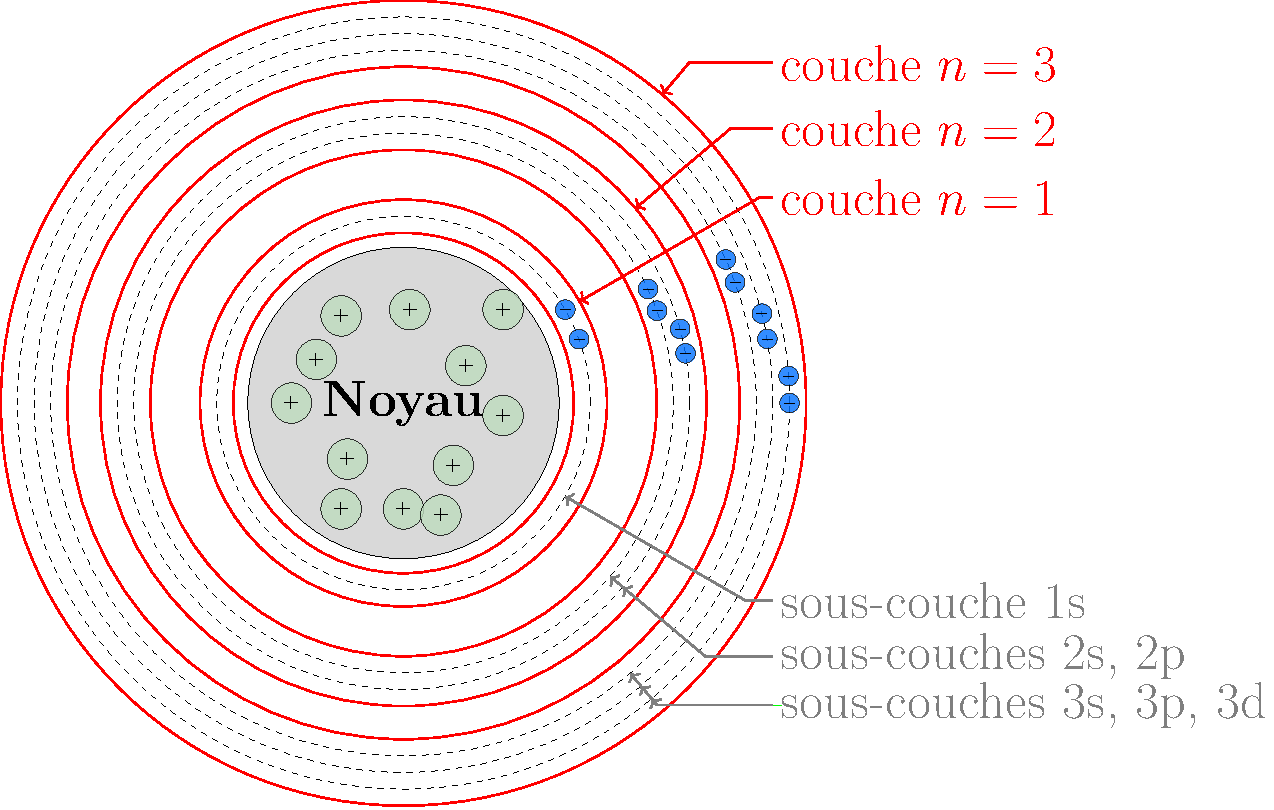
\includegraphics[width=.95\linewidth]{couchesquant}
		\captionof{figure}{Résumé fonctionnement OA.}
		\label{fig:couchesquant}
	\end{center}
\end{minipage}
\hfill
\begin{minipage}{0.45\linewidth}
	\centering
	\captionof{table}{Nombre maximal d'électron dans une sous-couche.}
	\label{tab:nbelecl}
	\begin{tabular}{lccccc}
		\toprule
		$\ell$     & 0 & 1 & 2  & 3  & 4
		\\\midrule
		Lettre     & s & p & d  & f  & g
		\\\midrule
		Nb. é. max & 2 & 6 & 10 & 14 & 18
		\\\bottomrule
	\end{tabular}
\end{minipage}

\subsection{Configuration électronique -- HP}
\subsubsection{Niveaux d'énergie}
On sait donc où peuvent se placer les électrons dans un atome, et on comprend
que plus il y a d'électrons plus on doit utiliser de couches différentes~: mais
comment se fait ce remplissage~? Est-ce qu'il est aléatoire, commence par la
fin…? Le critère se base sur un autre paramètre, celui du niveau d'énergie~:

\begin{tcb*}[cnt](prop){Règle de remplissage (partie 1)}
	Le remplissage des électrons dans un atome se fait par \textbf{niveau
		d'énergie croissant}. Autrement dit, on remplit les plus bas niveaux
	d'abord.
\end{tcb*}

Il faut donc parler du niveau d'énergie des électrons, et savoir comment ils
dépendent des nombres quantiques. On a, par définition,

\begin{tcb*}(defi){Niveaux d'énergie dans un atome}
	L'énergie d'un électron dans un atome ne dépend \textbf{que de $n$ et
		$\ell$}, mais \cancel{pas de $m_\ell$ ou $m_s$}, donc \textbf{ne dépend que
		de la sous-couche et pas de l'OA}. \bigbreak
	De plus, \textbf{l'énergie augmente avec $n+\ell$}.
\end{tcb*}

Ainsi, avec ces définitions et grâce à l'expérimentation, on arrive à une règle
empirique de remplissage~:

\begin{tcb*}(prop){Règle de remplissage de \textsc{Klechkowski}}
	\begin{center}
		\bfseries
		Les électrons d'un atome remplissent les différentes sous-couches à
		$n+\ell$ croissant, et pour deux valeurs égales de $n+\ell$, se fait à
		$n$ croissant.
	\end{center}
	\begin{minipage}{0.45\linewidth}
		\begin{figure}[H]
			\centering
			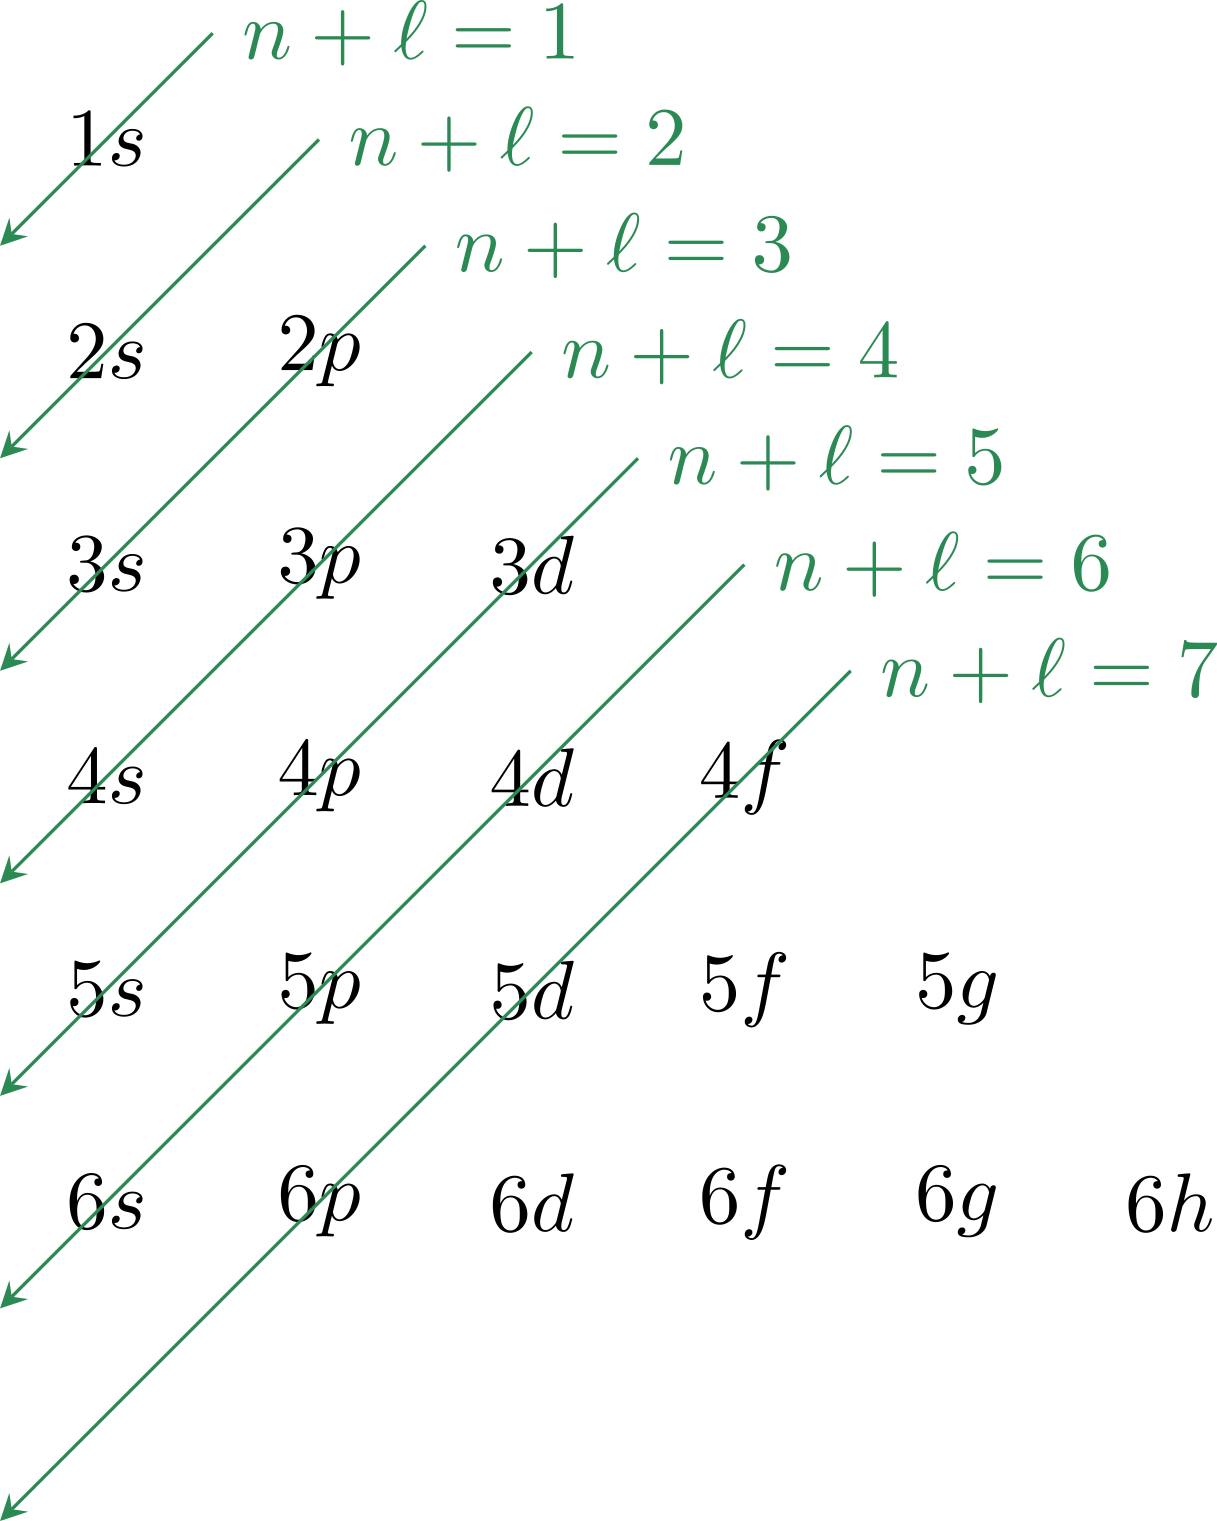
\includegraphics[scale=1]{klechkowski}
			\caption{Triangle de \textsc{Klechkowski}}
			\label{fig:klech}
		\end{figure}
	\end{minipage}
	\hfill
	\begin{minipage}{0.45\linewidth}
		On utilise alors une figure appelée le \textbf{triangle de
			\textsc{Klechkowski}} où on place les sous-couches dans un graphique avec
		$\ell$ en abscisse et $n$ en ordonnée~: le remplissage suit la ligne verte
		de haut en bas en diagonale. \bigbreak
		Ainsi, on remarque (mais il \textbf{faut savoir retrouver}) l'ordre de
		remplissage suivant~:
		\begin{center}
			1s\,2s\,2p\,3s\,3p\,4s\,3d\,4p\,5s\,4d\,5p…
		\end{center}
	\end{minipage}
\end{tcb*}

\begin{tcb*}[breakable](exem)<lftt>'l'{Configurations électroniques variées}
	Donner la configuration électronique de l'hydrogène ($Z = 1$), du carbone
	($Z = 6$), du phosphore ($Z = 15$), du fer ($Z=26$) et du plomb ($Z=82$).
	\tcblower
	On place les électrons (au nombre de $Z$) en remplissant les sous-couches au
	fur et à mesure dans l'ordre donné par la règle de \textsc{Klechkowski}~:
	\begin{itemize}[label=$\diamond$, leftmargin=20pt]
		\item $[\ce{H}]~: \elconf{H}$
		\item $[\ce{C}]~: \elconf{C}$
		\item $[\ce{P}]~: \elconf{P}$
		\item $[\ce{Fe}]~: \elconf{Fe}$
		\item $[\ce{Pb}]~: \elconf{Pb}$
	\end{itemize}
\end{tcb*}

\subsubsection{Supplément~: règle de \textsc{Hund} et cases quantiques}
La règle de \textsc{Pauli}, donnant le nombre maximal d'électrons dans une OA,
et la règle de \textsc{Klechkowski}, indiquant comment se construit le cortège
électronique d'un atome, ne permet pas de rendre compte de tous les phénomènes
observés. Notamment, si l'énergie individuelle d'un électron ne dépend en effet
pas de l'OA, il reste qu'ils peuvent avoir un effet de groupe, ce que traduit la
règle de \textsc{Hund}~:

\begin{tcb*}[cnt, bld](prop){Règle de \textsc{Hund}}
	Lors du remplissage des sous-couches, l'état le plus stable est
	celui où il y a un maximum de spin égaux (parallèles).
\end{tcb*}

Pour représenter le remplissage électronique, on peut symboliser les OA par des
cases «~quantiques~», représentant le nombre d'électrons dans chacune d'elle. Un
électron est alors représenté par une flèche, vers le haut ($\ua$) pour $m_s =
	+1/2$ et vers le bas ($\da$) sinon. Les sous-couches contenant plusieurs OA sont
représentées avec des cases collées les unes aux autres.

\begin{tcb*}(exem)<lftt>'l'{Représentations en cases quantiques}
	Par exemple, pour le phosphore de $Z=15$ et de configuration \elconf{P}~:
	\[
		\underset{\rm 1s^2}{\casea{\ua\da}}
		\quad
		\underset{\rm 2s^2}{\casea{\ua\da}}
		\quad
		\underset{\rm 2p^6}{\casec{\ua\da}{\ua\da}{\ua\da}}
		\quad
		\underset{\rm 3s^2}{\casea{\ua\da}}
		\quad
		\underset{\rm 3p^3}{\casec{\ua}{\ua}{\ua}}
	\]
	L'ordre des électrons dans la sous-couche 3p est obtenu par la règle de
	\textsc{Hund}~: on aurait en effet pu avoir
	\begin{align*}
		 & … \underset{\rm 3p^3}{\casec{\ua\da}{\ua}{\fa}}
		\\\text{ou}
		 & … \underset{\rm 3p^3}{\casec{\ua\da}{\da}{\fa}}
	\end{align*}
	Cependant, $\casec{\ua}{\ua}{\ua}$ est tout à fait équivalent à
	$\casec{\da}{\da}{\da}$~: il n'y a pas de discrimination sur la valeur des
	spins, juste sur leur parallélisme.
\end{tcb*}

% Cette configuration détaillée aura un impact sur les interactions entre atomes
% plus tard dans le chapitre. On note déjà quelques mots de vocabulaire~:

\begin{tcb*}(defi){Vocabulaire des OA}
	\begin{itemize}[label=$\diamond$, leftmargin=20pt]
		\item Deux électrons dans une même OA forment un \textbf{doublet}, on
		      dit qu'ils sont \textbf{appariés}.
		\item Un électron seul dans une OA est dit \textbf{célibataire}.
		\item Une OA vide est dite \textbf{vacante}.
	\end{itemize}
\end{tcb*}

\begin{tcb*}(rema)<lftt>'l'{\textsc{Hund} et exceptions}
	La règle de \textsc{Hund} peut parfois générer des exceptions à la règle de
	\textsc{Klechkowski}, mais la connaissance de ces exceptions est hors
	programme.
\end{tcb*}

\subsection{Électrons de cœur et de valence}
\subsubsection{Définition}

Les électrons des couches basses en énergie sont stables, très attirés par le
noyau et peu influencés par l'environnement de l'atome. Les électrons situés sur
l'extérieur sont en revanche moins liés au noyau plus sensibles à
l'environnement de l'atome~: ce sont eux qui sont à l'origine des propriétés
chimiques de l'atome et susceptibles de former des liaisons chimique ou former
des ions. Leur caractéristique particulière amène à nom particulier~:

\begin{tcb*}(defi){Électrons de cœur et de valence}
	\psw{
		Les électrons de \textbf{valence} sont les \textbf{électrons de la dernière
			couche} occupée, ainsi que \textbf{les sous-couches partiellement remplies}.
		Les électrons de cœur sont tous les autres.
		\bigbreak
		Pour $Z \leq 18$, on retiendra que les électrons de valence sont \ul{ceux
			sur la couche de plus grand $n$}.
	}
\end{tcb*}

\begin{tcb*}(exem)<lftt>'l'{Électrons de cœur et de valence}
	\begin{itemize}[label=$\diamond$, leftmargin=20pt]
		\bitem{Pour le carbone}~:
		\[[\ce{C}]~:
			\underbracket[1pt]{\strut \rm 1s^2}_{\text{cœur}}
			\underbracket[1pt]{\strut \rm \color{red}2s^22p^2}_{\text{valence}}\]
		La dernière couche occupée est $n=2$, donc on compte les
		sous-couches 2s et 2p. La sous-couche partiellement
		remplie 2p est déjà comptée dans la plus grande couche. On compte
		donc $2+2=4$ électrons de valence.
		\bitem{Pour le fer}~:
		\[[\ce{Fe}]~:
			\underbracket[1pt]{\strut \elconf{Ar}}_{\text{cœur}}
			\underbracket[1pt]{\strut \rm \color{red}4s^23d^6}_{\text{valence}}\]
		La dernière couche occupée est $n=4$, on compte donc la sous-couche
		4s. La sous-couche partiellement remplie est la 3d. On a donc $2+6 =
			8$ électrons de valence.
		\bitem{Pour le brome}~:
		\[[\ce{Br}]~: \rm
			\underbracket[1pt]{\strut \elconf{Ar}}_{\heartsuit}
			\underbracket[1pt]{\strut \rm \color{red}4s^2}_{\rm V}
			\underbracket[1pt]{\strut \rm \color{black}3d^{10}}_{\heartsuit}
			\underbracket[1pt]{\strut \rm \color{red}4p^5}_{\rm V}\]
		La dernière couche occupée est $n=4$, on compte donc les
		sous-couches 4s et 4p. La sous-couche 4p partiellement remplie est
		déjà comptabilisée, la 3d étant pleine. On a donc $2+5=7$ électrons
		de valence.
	\end{itemize}
\end{tcb*}

\subsubsection{Stabilité et ions}

Cette étude des électrons de valence fait alors apparaître un dernier critère de
stabilité~:
% , semblable à la règle de \textsc{Hund} mais qui n'est qu'empirique~:
\vspace{-10pt}
\begin{tcb*}(ror){Critère de stabilité}
	\vspace{-15pt}
	\psw{
		\begin{center}
			Les édifices les plus stables sont ceux dont la couche de valence se
			termine par une sous-couche p \textbf{totalement remplie}.
		\end{center}
	}
	On le reverra par la suite, ces éléments sont ceux des gaz rares.
\end{tcb*}

Ainsi, un atome sera susceptible de former un ion qui assure sa stabilité en
saturant sa couche de valence.

\begin{tcb*}(exem)<lftt>'l'{Stabilité d'édifices atomiques bloc p}
	\begin{itemize}[label=$\diamond$, leftmargin=20pt]
		\bitem{Fluor}~:
		\[[\ce{F}]~: \elconf{F}\]
		En rajoutant un électron, la sous-couche 2p sera saturée, et on
		obtient la configuration électronique du néon. Le fluor sera donc
		susceptible de facilement former l'ion \ce{F-}.
		\bitem{Sodium}~:
		\[[\ce{Na}]~: \elconf{Na}\]
		En enlevant l'électron sur 3s, on obtient ici encore la
		configuration électronique du néon. On formera donc l'ion \ce{Na+}.
	\end{itemize}
\end{tcb*}

Les cas avec des sous-couches 3d sont plus complexes à prévoir.

\section{Tableau périodique}

La première classification a été proposée par Dmitri \textsc{Mendeleïev} en
1869. À l'époque, 63 éléments étaient connus et des analogies de propriétés
physico-chimiques (réactivité, changement d'état, etc.) avaient été notées.
\textsc{Mendeleïev} a proposé un classement dans un tableau tel que les éléments
y soient ordonnés par masse croissante et surtout que les éléments ayant des
propriétés semblables soient rangés les uns au dessus des autres.

Le génie de \textsc{Mendeleïev} a été de faire primer les propriétés
physico-chimiques sur le classement par masse croissante. Il a ainsi inversé la
place de certains éléments pour maintenir l'unité des propriétés parmi les
colonnes, et pensé à laisser des places vides. Cela a permis de prédire les
propriétés de certains éléments pas encore connus à l'époque… et donc de les
découvrir~! À ce jour, 118 éléments sont connus dont 94 sont naturels. Seuls 80
d'entre eux sont stables, les autres se désintègrent spontanément (et plus ou
moins rapidement) par radioactivité.

\subsection{Construction}
La construction du tableau repose sur la configuration électronique~:

\begin{tcb*}[cnt](defi){Construction du tableau}
	\psw{
		Dans le tableau périodique, les éléments chimiques sont rangés par
		\textbf{numéro atomique} $Z$ \textbf{croissant}, et de telle sorte à ce
		que les \textbf{atomes de même configuration de valence} soient
		\textbf{dans la même colonne}.
	}
\end{tcb*}
Une seule exception~: l'hélium, de configuration électronique 1s$^2$, est dans
la colonne p$^6$ avec tous les éléments ayant une couche externe complète.
\bigbreak
Par conséquent, en passant d'une ligne à une autre on augmente le nombre
quantique principal d'une unité~; corollairement les éléments d'une \textbf{même
	ligne} on le \textbf{même nombre quantique principal}. Un tableau périodique
interactif est disponible en ligne\footnote{\url{https://ptable.com/}}.

% \begin{tcb*}(exem)<lftt>'l'{Repérage dans le tableau}
% 	L'azote a pour numéro atomique $Z_{\ce{N}}=7$. Écrire sa configuration
% 	électronique. Dans le tableau périodique, il se trouve à droite du carbone,
% 	et au-dessus du phosphore. En déduire leur numéro atomique et leur
% 	configuration.
% 	\tcblower
% 	\begin{itemize}[label=$\diamond$]
% 		\item $[\ce{N}]~: \elconf{N}$.
% 		\item  \ce{C} à gauche de \ce{N} $\Ra Z_{\ce{C}} = Z_{\ce{N}} - 1 = 6$, d'où
% 		      $[\ce{C}]~: \elconf{C}$.
% 		\item \ce{P} en-dessous de \ce{N} donc on augmente le nombre quantique
% 		      principal de la configuration externe de \ce{N} par 1 pour passer de
% 		      2s$^3$ à 2p$^3$. On en déduit la configuration complète en
% 		      remplissant dans l'ordre~: $[\ce{P}]~: \elconf{P}$ et on compte
% 		      $Z_{\ce{P}} = 15$.
% 	\end{itemize}
% \end{tcb*}

\subsection{Blocs}

\begin{tcb*}(defi){Bloc du tableau}
	\psw{
		\begin{center}
			On appelle bloc du tableau périodique l'ensemble des éléments pour
			lesquels la sous-couche non-complètement remplie est la même.
		\end{center}
		Ils correspondent visuellement aux décrochages dans la structure du tableau,
		cf.\ Figure~\ref{fig:tabper}.
	}
\end{tcb*}

\begin{figure}[htbp]
	\centering
	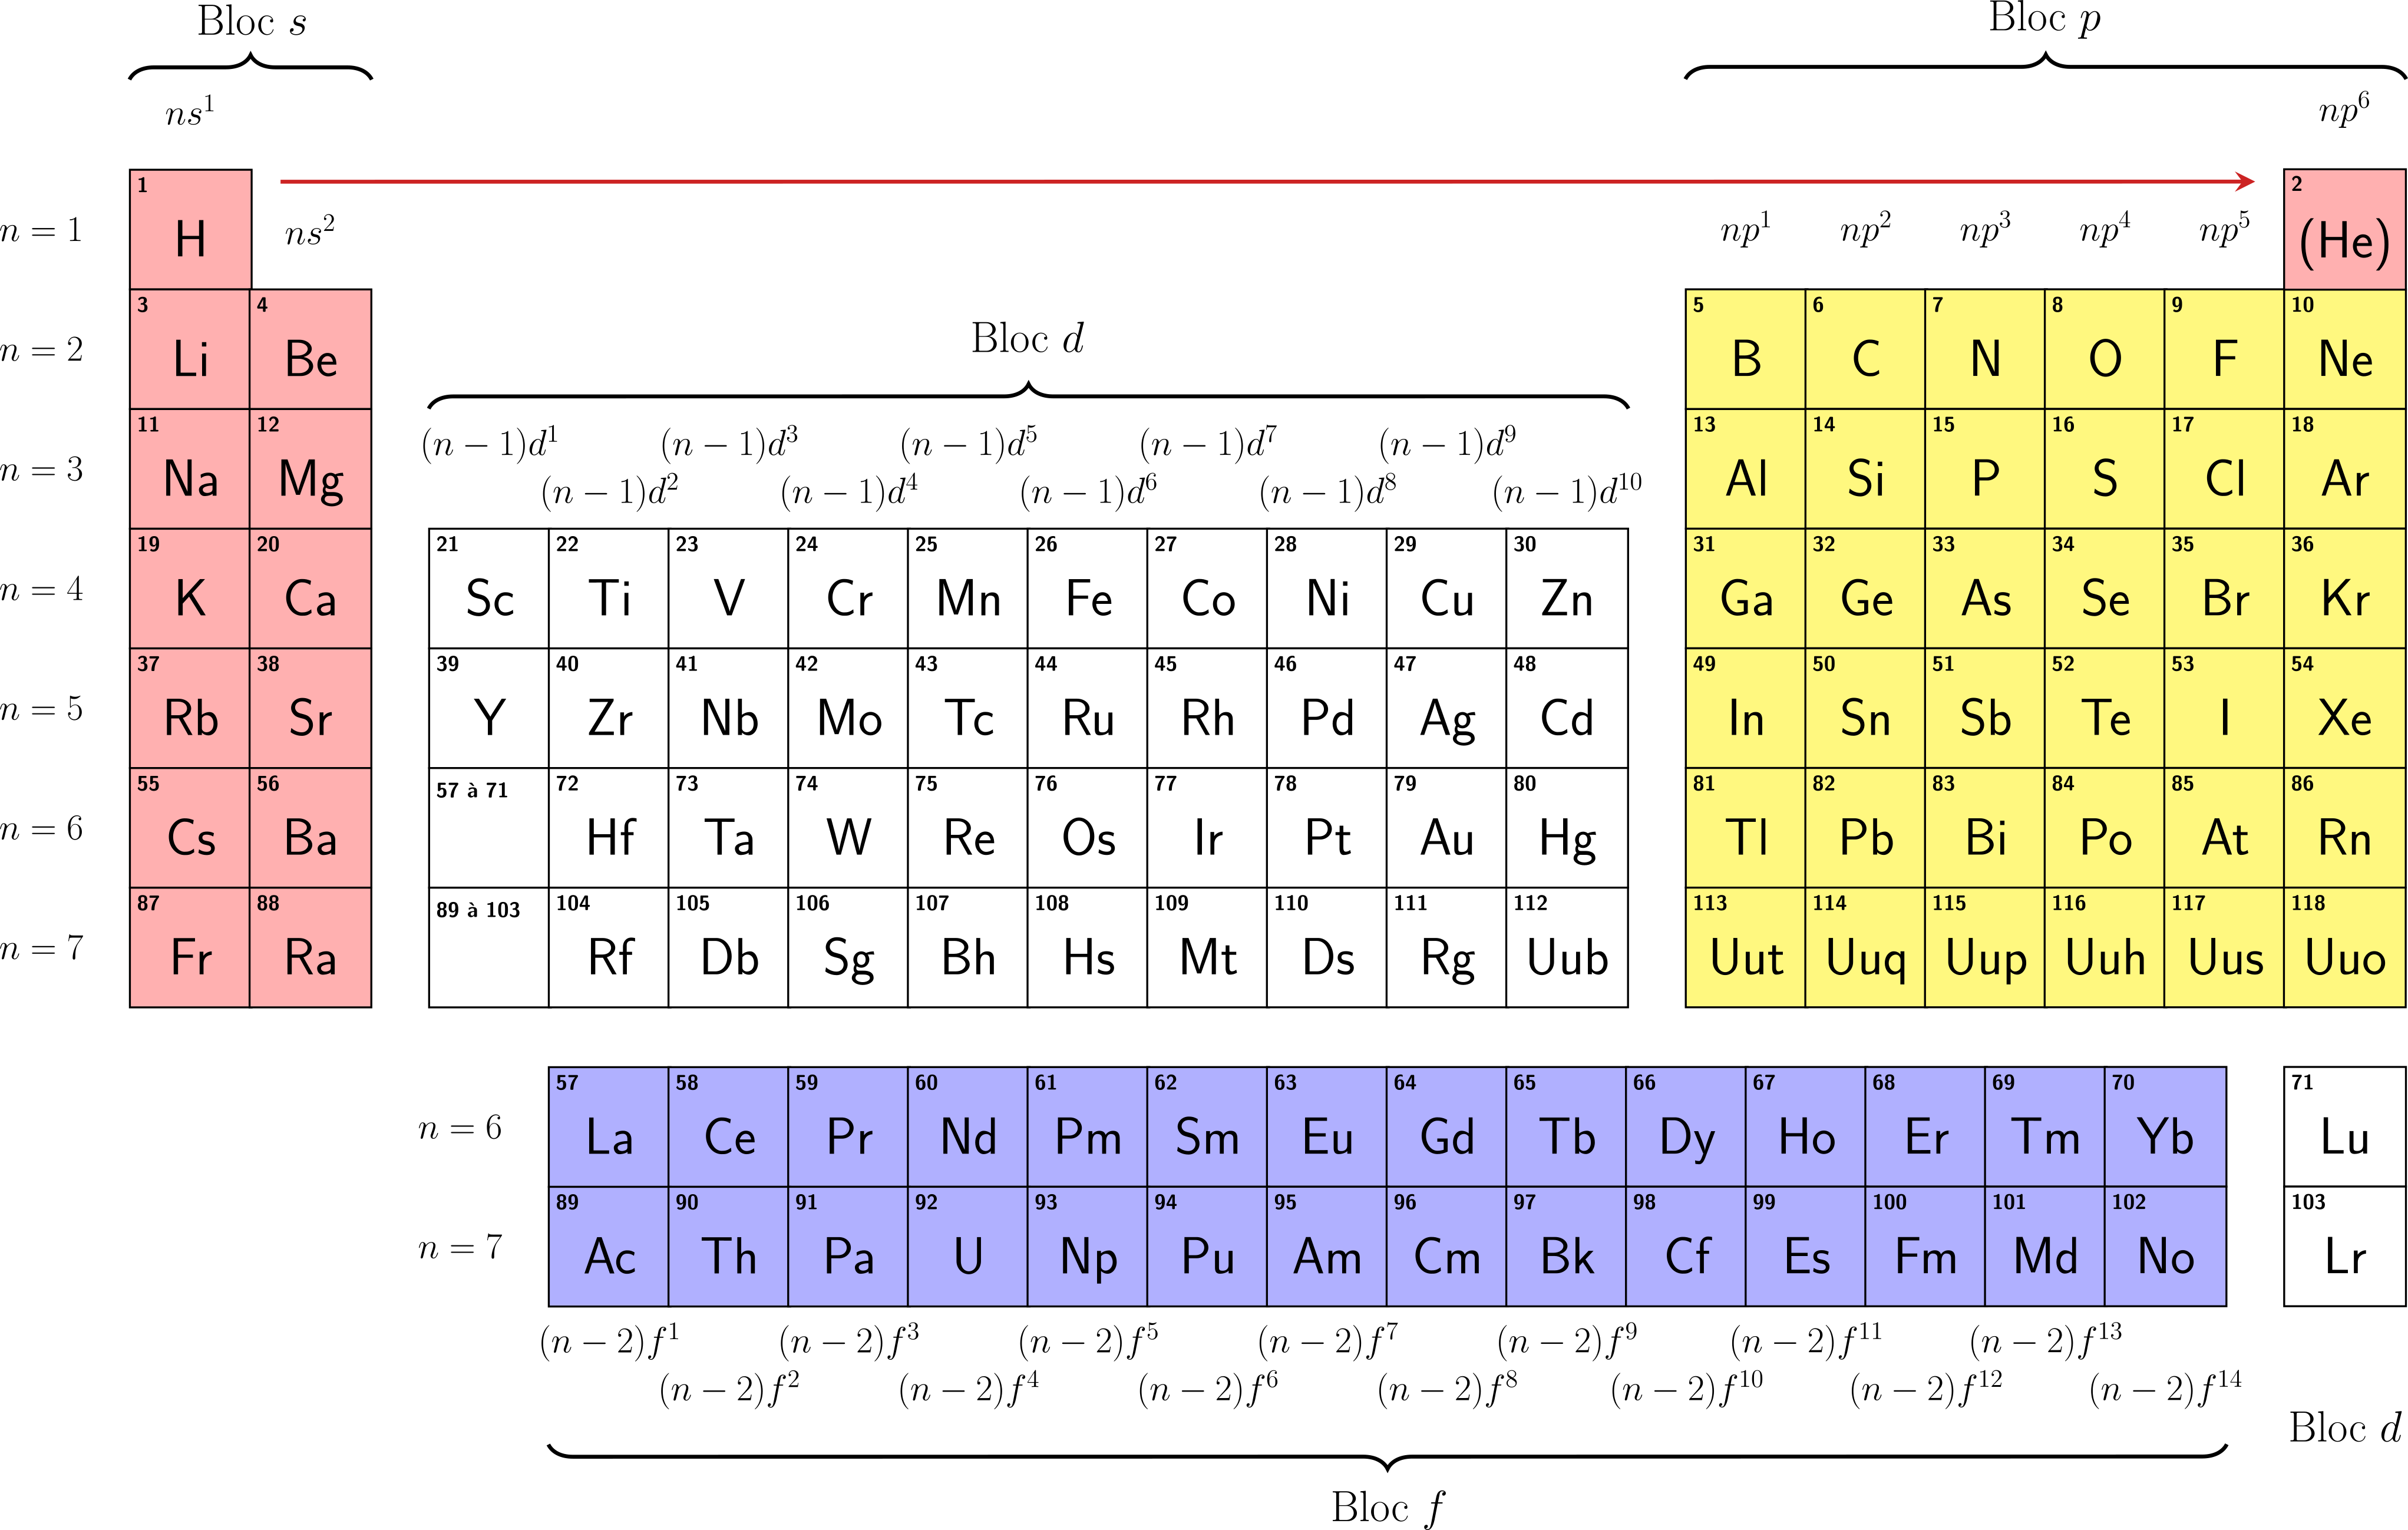
\includegraphics[width=\linewidth]{tab_per}
	\caption{Structure du tableau périodique. La configuration de la sous-couche
		la plus externe de l'atome est indiquée en tête de chaque colonne~; la
		valeur maximale de $n$ est donnée à gauche de chaque ligne. Les différentes
		couleurs de fond sont associées au différents blocs du tableau.}
	\label{fig:tabper}
\end{figure}

On considère ainsi le plus souvent que le tableau périodique a \textbf{18
	colonnes}, puisqu'on a l'habitude de placer le bloc f en-dessous du tableau par
souci de place. Ces colonnes sont celles des blocs, on a la correspondance
suivante~:

\begin{table}[htbp]
	\centering
	\caption{Correspondance blocs, tableau et valence.}
	\label{tab:btv}
	\begin{tabularx}{\linewidth}{lYYYYYYYYYYYYYYYYYY}
		\toprule
		                                      &
		\multicolumn{2}{c}{\bfseries Bloc s}  &
		\multicolumn{10}{c}{\bfseries Bloc d} &
		\multicolumn{6}{c}{\bfseries Bloc p}
		\\\cmidrule(lr){2-3} \cmidrule(lr){4-13} \cmidrule(lr){14-19}
		                                      &
		\multicolumn{2}{c}{2 él.}             &
		\multicolumn{10}{c}{10 éléments}      &
		\multicolumn{6}{c}{6 éléments}
		\\\midrule
		Valence                               & s$^1$ & s$^2$ & d$^1$ & d$^2$    & d$^3$ & d$^4$ & d$^5$ & d$^6$
		                                      & d$^7$ & d$^8$ & d$^9$ & d$^{10}$ & p$^1$ & p$^2$ & p$^3$ &
		p$^4$                                 & p$^5$ & p$^6$
		\\
		Colonne                               & 1     & 2     & 3     & 4        & 5     & 6     & 7     & 8     & 9 & 10 & 11 & 12 & 13 & 14 &
		15                                    & 16    & 17    & 18
		\\\bottomrule
	\end{tabularx}
\end{table}

\subsubsection{Position dans la classification}

On peut ainsi placer un élément dans le tableau connaissant sa configuration
électronique~:
\begin{itemize}
	\item Le carbone a pour configuration
	      \[[\ce{C}]~: \elconf{C}\]
	      Le plus grand nombre est $n=2$, il est donc sur la deuxième ligne. Sa
	      configuration termine par 2p$^2$~: il est sur la 14\ieme\ colonne.
	\item L'or a pour configuration
	      \[[\ce{Au}]~: \elconf{Au}\]
	      Le plus grand nombre est $n=6$, il est donc sur la sixième ligne. Sa
	      configuration se termine par 3d$^9$, il est sur la 11\ieme\ colonne.
\end{itemize}

\subsubsection{Valence à partir de la position}

À l'inverse, on peut retrouver la configuration de valence d'un atome du bloc s
ou p à partir de ses coordonnées~:
\begin{itemize}
	\item Le numéro de ligne donne le $n$ de valence~;
	\item Le numéro de colonne permet d'obtenir le nombre d'électrons de
	      valence.
\end{itemize}
Si le bloc $d$ rentre en compte, ça se complique.

\begin{tcb*}(ror){Valence à partir de la position}
	\begin{center}
		\captionof{table}{Électrons de valence des blocs $s$ et $p$.}
		\label{tab:valsp}
		\begin{tabular}{lcccccccc}
			\toprule
			                                    &
			\multicolumn{2}{c}{\textbf{Bloc s}} &
			\multicolumn{6}{c}{\textbf{Bloc p}}
			\\ \cmidrule(lr){2-3} \cmidrule(lr){4-9}
			Colonne                             & 1      & 2      & 13           & 14           & 15           & 16           & 17           & 18
			\\\midrule
			Config.\ valence                    & ns$^1$ & ns$^2$ & ns$^2$np$^2$ & ns$^2$np$^2$ & ns$^2$np$^3$ & ns$^2$np$^4$ & ns$^2$np$^5$ & ns$^2$np$^6$
			\\\midrule
			Nb. é.\ valence                     & 1      & 2      & 3            & 4            & 5            & 6            & 7            & 8
			\\\bottomrule
		\end{tabular}
	\end{center}
\end{tcb*}


\subsection{Analyse par période}
\begin{tcb*}(defi){Période du tableau périodique}
	\psw{
		On appelle \textbf{période} une \textbf{ligne} de la classification
		périodique. Les éléments d'une \textbf{même période} ont la \textbf{même}
		configuration de \textbf{cœur}, mais des configurations de \textbf{valence
			différentes}.
	}
\end{tcb*}

Pour avoir le nombre d'éléments par période, on reprend le triangle de
\textsc{Klechkowski}~:
\begin{itemize}
	\bitem{Période 1}~: remplissage progressif du niveau 1s, donc 2 éléments.
	\bitem{Périodes 2 et 3}~: remplissage des niveaux $n$s et $n$p, donc $2+6=8$
	éléments.
	\bitem{Périodes 4 et 5}~: remplissage des niveaux $n$s, $(n-1)$d et $n$p, donc
	$2+10+6=18$ éléments.
\end{itemize}

\begin{tcb*}(ror){Moyen mnémotechnique pour les 2 premières périodes}
	Il vous est demandé de connaître l'ordre des éléments des périodes 2 et 3. On
	pourra pour cela utiliser les phrases mnémotechniques~:
	\begin{itemize}
		\bitem{Première période}~:
		$\overset{\text{Lithium}}{\textbf{Li}\text{ly}}
			\,\,
			\overset{\text{Béryllium}}{\textbf{Be}\text{rçait}}
			\,\,
			\overset{\text{Bore}}{\textbf{B}\text{oris}}
			\,\,
			\overset{\text{Carbone}}{\textbf{C}\text{hez}}
			\,\,
			\overset{\text{Azote}}{\textbf{N}\text{otre}}
			\,\,
			\overset{\text{Oxygène}}{\textbf{O}\text{ncle}}
			\,\,
			\overset{\text{Fluor}}{\textbf{F}\text{lorent}}
			\,\,
			\overset{\text{Néon}}{\textbf{Ne}\text{stor}}$
		\bitem{Deuxième période}~:
		$\overset{\text{Sodium}}{\textbf{Na}\text{poléon}}
			\,\,
			\overset{\text{Magnésium}}{\textbf{M}\text{an}\textbf{g}\text{ea}}
			\,\,
			\overset{\text{Aluminium}}{\textbf{Al}\text{lègrement}}
			\,\,
			\overset{\text{Silicium}}{\textbf{Si}\text{x}}
			\,\,
			\overset{\text{Phosphore}}{\textbf{P}\text{anais}}
			\,\,
			\overset{\text{Soufre}}{\textbf{S}\text{ans}}
			\,\,
			\overset{\text{Chlore}}{\textbf{Cl}\text{aquer}}
			\,\,
			\text{d'}
			\overset{\text{Argon}}{\textbf{Ar}\text{tère}}$
	\end{itemize}
\end{tcb*}

\subsection{Analyse par famille}
\begin{tcb*}(defi){Famille du tableau périodique}
	\psw{
		On appelle \textbf{famille} une \textbf{colonne} de la classification. Tous
		les éléments d'une \textbf{même famille} on la \textbf{même} configuration
		de \textbf{valence}, mais des configurations de \textbf{cœur différentes}.
	}
\end{tcb*}
Conformément au mode de construction de \textsc{Mendeleïev}, les éléments d'une
même famille ont des propriétés chimiques semblables~: ces propriétés sont
déterminées par la configuration de valence.

\subsubsection{Gaz nobles}
Il s'agit de la colonne la plus à droite du tableau périodique : hélium, néon,
argon, krypton, xénon, radon. Les gaz nobles se caractérisent par une
sous-couche externe complètement remplie, ce qui leur confère une très grande
stabilité. Ils sont donc quasiment inertes chimiquement : ils ne participent à
aucune transformation. \bigbreak

Par échanges d'électrons, les éléments tendent à se \textbf{rapprocher de la
	configuration électronique du gaz noble le plus proche}.

\subsubsection{Halogènes}
Il s'agit de l'avant-dernière colonne du tableau périodique : fluor, chlore,
brome, iode, astate. Leur configuration de valence est en np$^5$, il ne leur
manque donc qu'un électron pour en avoir le même nombre que le gaz noble qui les
suit et saturer leur couche de valence. En particulier, ils ont des facilités à
former des \textbf{anions} chargés une fois (\ce{F-}, \ce{Cl-}, \ce{Br-},
\ce{I-}), et sont des oxydants forts.

\subsubsection{Métaux alcalins}
Il s'agit de la colonne la plus à gauche du tableau périodique, dont l'hydrogène
est souvent mis à part : lithium, sodium, potassium, rubidium, césium. Leur
configuration de valence est en ns$^1$, ils ont donc simplement un électron de
plus par rapport au gaz noble qui les précède. Ils ont donc des facilités à
former des cations chargés une fois (\ce{Li+}, \ce{Na+}, \ce{K+}), et sont des
réducteurs forts.

\subsubsection{Métaux alcalino-terreux}
C'est la deuxième colonne~: béryllium, magnésium, calcium, strontium, baryum et
radium. Leur configuration de valence est en ns$^{2}$, et ont donc 2 électrons
de plus que le gaz noble les précédant. Ils forment des cations chargés deux
fois (\ce{Be2+}, \ce{Mg2+}, \ce{Ca2+}) et sont des réducteurs forts.

\subsubsection{Métaux}
Ce n'est pas une famille à proprement parler, puisqu'ils ne correspondent pas à
une colonne en particulier. Les métaux sont des solides aux conditions usuelles
de température et de pression (sauf le mercure), et sont définis par le fait que
ce sont de \textbf{bons conducteurs électriques}, susceptibles de fournir des
électrons à la conduction car retiennent peu leurs électrons. Entre métaux et
non-métaux, il y a les semi-conducteurs.

\begin{center}
	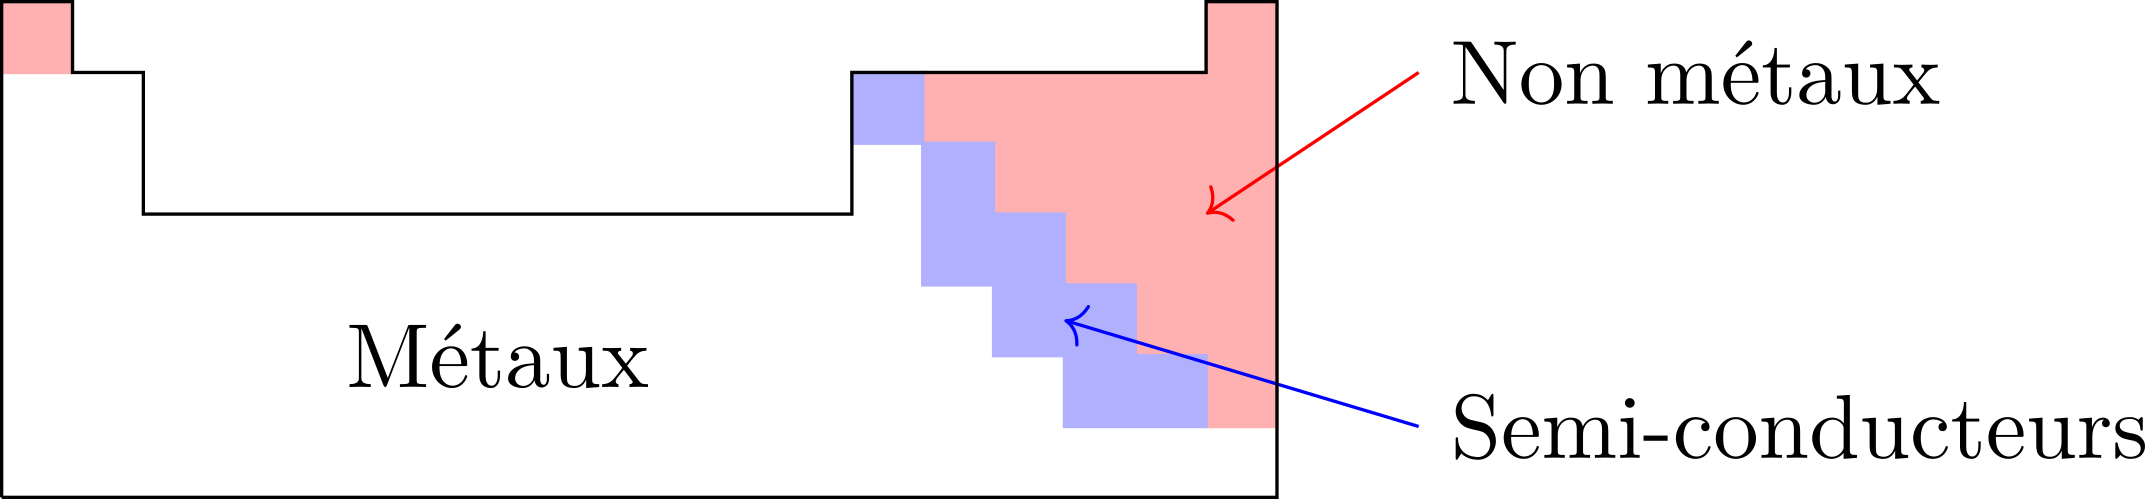
\includegraphics[scale=1]{metaux}
\end{center}

\section{Structure électronique des molécules}

Les atomes peuvent se lier entre eux au sein de molécules ou d'ions
polyatomiques. Il existe plusieurs modèles pour décrire ces
interactions entre atomes au sein des molécules~; ici nous détaillons le modèle
de \textsc{Lewis} (début \textsc{xx}\ieme), un modèle très simple mais efficace.

\subsection{Représentation de \textsc{Lewis} des atomes}
Rappelons encore une fois que les électrons de valence correspondent aux
électrons situés dans la dernière couche occupée de l'atone.
Ils forment donc sa partie extérieure, et sont ceux qui peuvent interagir avec
les atomes voisins.

\begin{tcb*}(defi){Représentation de \textsc{Lewis}}
	Dans la représentation de \textsc{Lewis}, on représente les électrons de
	valence~:
	\begin{itemize}
		\item \psw{
			      Par un tiret pour un doublet d'électrons (OA pleine)~;
		      }
		\item \psw{
			      Par un point pour un électron célibataire (OA un seul électron)~;
		      }
		\item \psw{
			      Par un rectangle pour une OA vide.
		      }
	\end{itemize}
\end{tcb*}

\begin{tcb*}(exem)<lftt>'l'{Représentations de \textsc{Lewis} classiques}
	\begin{minipage}{0.48\linewidth}
		\begin{gather*}
			\ce{H}~:
			\quad
			\underset{\rm 1s^1}{\casea{\ua}}
			\quad
			\hlew{0}
			\\
			\ce{C}~:
			\quad
			\underset{\rm 1s^2}{\casea{\ua\da}}
			\qquad
			\underset{\rm 2s^2}{\casea{\ua\da}}
			\qquad
			\underset{\rm
				2p^2}{\casec{\ua\tikzmark{T1}}{\ua\tikzmark{T2}}{\fa\tikzmark{T3}}}
			\quad
			\lewis{0.2|46.,C}\tikzmark{C}
		\end{gather*}
	\end{minipage}
	\hfill
	\begin{minipage}{0.48\linewidth}
		\begin{gather*}
			\ce{N}~:
			\quad
			\underset{\rm 1s^2}{\casea{\ua\da}}
			\qquad
			\underset{\rm 2s^2}{\casea{\ua\da}}
			\qquad
			\underset{\rm 2p^3}{\casec{\ua}{\ua}{\ua}}
			\quad
			\nlew{4}
			\\
			\ce{O}~:
			\quad
			\underset{\rm 1s^2}{\casea{\ua\da}}
			\qquad
			\underset{\rm 2s^2}{\casea{\ua\da}}
			\qquad
			\underset{\rm 2p^4}{\casec{\ua\da}{\ua}{\ua}}
			\quad
			\lewis{0.246.,O}
		\end{gather*}
	\end{minipage}
\end{tcb*}

\tikz[remember picture, overlay]
\draw[->, transform canvas={xshift=-5pt, yshift=-3pt}, shorten >=3pt]
(pic cs:T1) to[out=-70, in=-90] (pic cs:C)
;
\tikz[remember picture, overlay]
\draw[->, transform canvas={xshift=-5pt, yshift=1pt}, shorten >=3pt]
(pic cs:T2) to[out=-70, in=-90] ([shift={(6pt,0)}]pic cs:C)
;
\tikz[remember picture, overlay]
\draw[->, transform canvas={xshift=-5pt, yshift=2pt}, shorten >=3pt]
([shift={(-42pt,0)}]pic cs:T1) to[out=70, in=180] ([shift={(-6pt,0)}]pic cs:C)
;
\tikz[remember picture, overlay]
\draw[->, transform canvas={xshift=0pt, yshift=10pt}, shorten >=3pt]
(pic cs:T3) to[out=70, in=90] ([shift={(-5pt,1.5pt)}]pic cs:C)
;

C'est ici que la règle de \textsc{Hund} joue un rôle, puisqu'on voit qu'avec 6
électrons de valence on n'obtient \textbf{pas} 6 électrons célibataires. Elle ne
suffit cependant pas à tout expliquer~; notamment, le carbone ne se retrouve pas
avec une lacune dans sa configuration de \textsc{Lewis} usuelle, parce qu'on le
trouve dans un état plus stable sous la forme suivante~:

\[
	\ce{C}~:
	\quad
	\underset{\rm 1s^2}{\casea{\ua\da}}
	\qquad
	\underset{\rm 2s^1}{\casea{\ua}}
	\qquad
	\underset{\rm
		2p^2}{\casec{\ua\tikzmark{Tt1}}{\ua\tikzmark{Tt2}}{\ua\tikzmark{Tt3}}}
	\quad
	\clew\tikzmark{Cc}
\]
\tikz[remember picture, overlay]
\draw[->, transform canvas={xshift=-5pt, yshift=-3pt}, shorten >=3pt]
(pic cs:Tt1) to[out=-70, in=-90] (pic cs:Cc)
;
\tikz[remember picture, overlay]
\draw[->, transform canvas={xshift=-5pt, yshift=1pt}, shorten >=3pt]
(pic cs:Tt2) to[out=-70, in=-90] ([shift={(6pt,0)}]pic cs:Cc)
;
\tikz[remember picture, overlay]
\draw[->, transform canvas={xshift=-5pt, yshift=2pt}, shorten >=3pt]
([shift={(-42pt,0)}]pic cs:Tt1) to[out=70, in=180] ([shift={(-6pt,0)}]pic
cs:Cc)
;
\tikz[remember picture, overlay]
\draw[->, transform canvas={xshift=0pt, yshift=10pt}, shorten >=3pt]
(pic cs:Tt3) to[out=70, in=90] ([shift={(-5pt,1.5pt)}]pic cs:Cc)
;

\vspace{-15pt}
\begin{tcb*}(ror){Représentations à retenir}
	D'une manière générale et ce pour $Z \leq 18$, on peut retenir qu'on
	organise les électrons de valence autour des 4 «~côtés~» d'un élément,
	électron par électron~:
	\begin{center}
		\captionof{table}{Schémas de \textsc{Lewis} des blocs $s$ et $p$.}
		\label{tab:lewissp}
		\begin{tabular}{lcccccccc}
			\toprule
			                                    &
			\multicolumn{2}{c}{\textbf{Bloc s}} &
			\multicolumn{6}{c}{\textbf{Bloc p}}
			\\ \cmidrule(lr){2-3} \cmidrule(lr){4-9}
			Colonne                             & 1
			                                    & 2                  & 13 & 14 & 15 & 16 & 17 & 18
			\\\midrule
			Nb. é.\ valence                     & 1                  & 2  & 3  & 4  & 5  & 6  & 7  & 8
			\\\midrule
			Schéma                           &
			\lewis{0.,X}                        & \lewis{0.2.,X}     &
			\lewis{0.2.4.,X}                    & \lewis{0.2.4.6.,X} &
			\lewis{02.4.6.,X}                   & \lewis{024.6.,X}   &
			\lewis{0246.,X}                     & \lewis{0246,X}
			\\\bottomrule
		\end{tabular}
	\end{center}
	On retiendra notamment les représentations de \textsc{Lewis} des atomes
	d'hydrogène, de carbone, d'azote, d'oxygène et de fluor~:
	\[
		\lewis{0.,H}
		\qquad
		\lewis{0.2.4.6.,C}
		\qquad
		\lewis{0.2.46.,N}
		\qquad
		\lewis{0.2.46,O}
		\qquad
		\lewis{0.246,F}
	\]
\end{tcb*}

\subsection{Liaison covalente}
\subsubsection{Introduction}
Une couche de valence pleine apporte de la stabilité à l'atome~; pour
l'atteindre, les métaux ont tendance à perdre des électrons (car leur énergie
d'ionisation est faible), et les non-métaux ont plutôt tendance à gagner des
électrons~: ils peuvent former des anions ou partager des électrons.

\begin{tcb*}(defi){Liaison covalente}
	\psw{
		Une \textbf{liaison covalente} ou \textbf{doublet liant} est la mise en
		commun de deux électrons de valence entre deux atomes. Les deux atomes liés
		sont alors à une plus faible distance que lorsqu'ils étaient séparés, et
		cette distance est fixe.
	}
\end{tcb*}

\begin{tcb*}(exem)<lftt>'l'{Liaisons covalentes classiques}
	\vspace{-12pt}
	\psw{
		\begin{gather*}
			\ce{\Lewis{0.,H} \qquad \Lewis{4.,H} -> \cfig{H-H}}
			\\
			\ce{\Lewis{0:35,O} \qquad \Lewis{14:7,O} ->
				\cfig{\Lewis{35,O}=\Lewis{17,O}}}
		\end{gather*}
	}
	\vspace{-30pt}
\end{tcb*}

Le trait symbolise le partage de deux électrons entre deux atomes. Il se peut
que le partage ne soit pas équitable, et qu'un atome ait apporté les deux
électrons et l'autre aucun. Deux atomes peuvent mettre en commun plus de deux
électrons~: on a alors une liaison multiple.

\subsubsection{Longueur et énergie de la liaison covalente}

Lors de cette interaction, il y a à la fois attraction entre les électrons de
valence d'un atome et le noyau positif de l'autre, mais aussi répulsion entre
les nuages électroniques. Il existe une distance entre les noyaux pour laquelle
le système est dans un état d'équilibre stable, ce qui correspond à la longueur
d'une liaison covalente. Représentons ci-dessous l'allure du graphique d'énergie
potentielle associée à l'interaction entre deux atomes liés,
Figure~\ref{fig:lgcov}.

\begin{figure}[htbp]
	\centering
	\sswitch{
		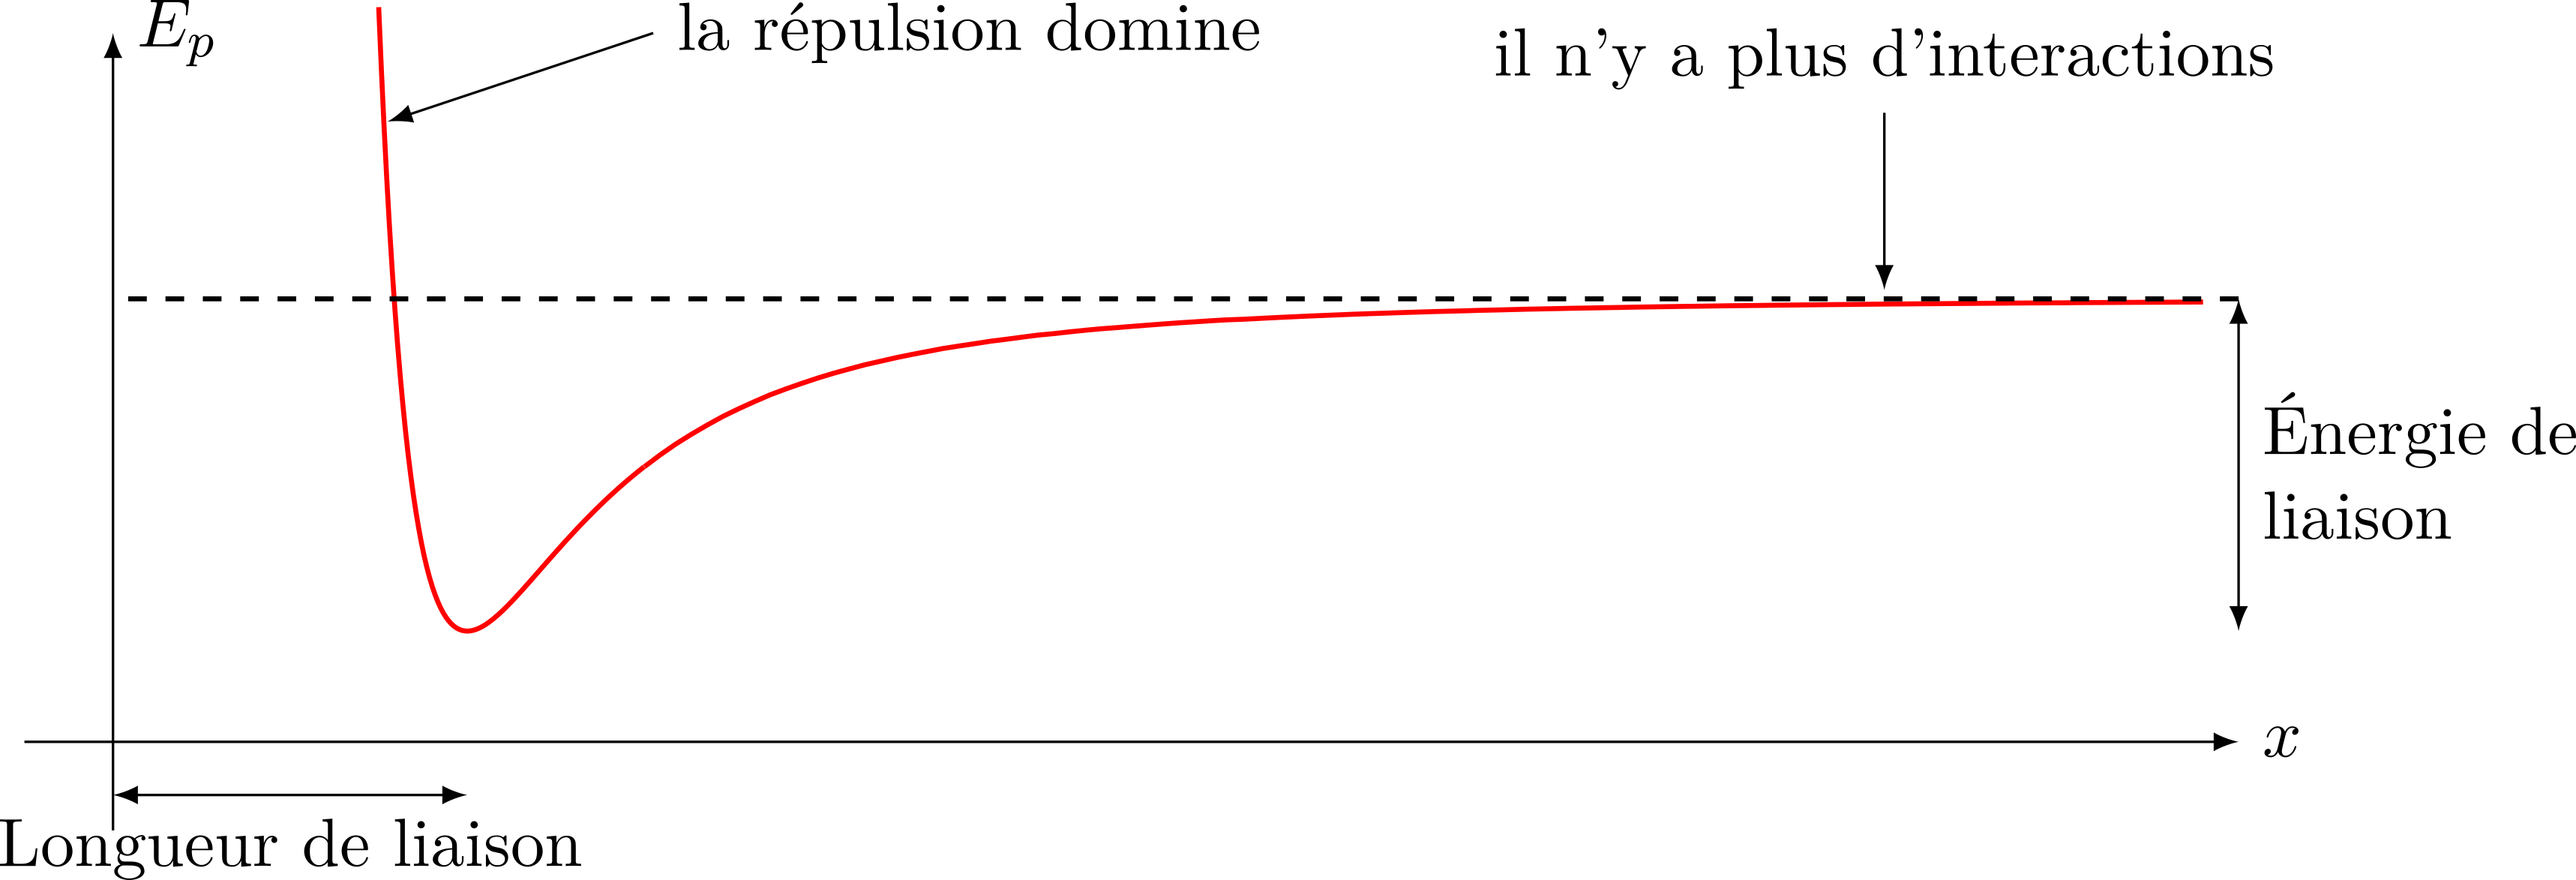
\includegraphics[scale=1, draft=true]{lgcov}
	}{
		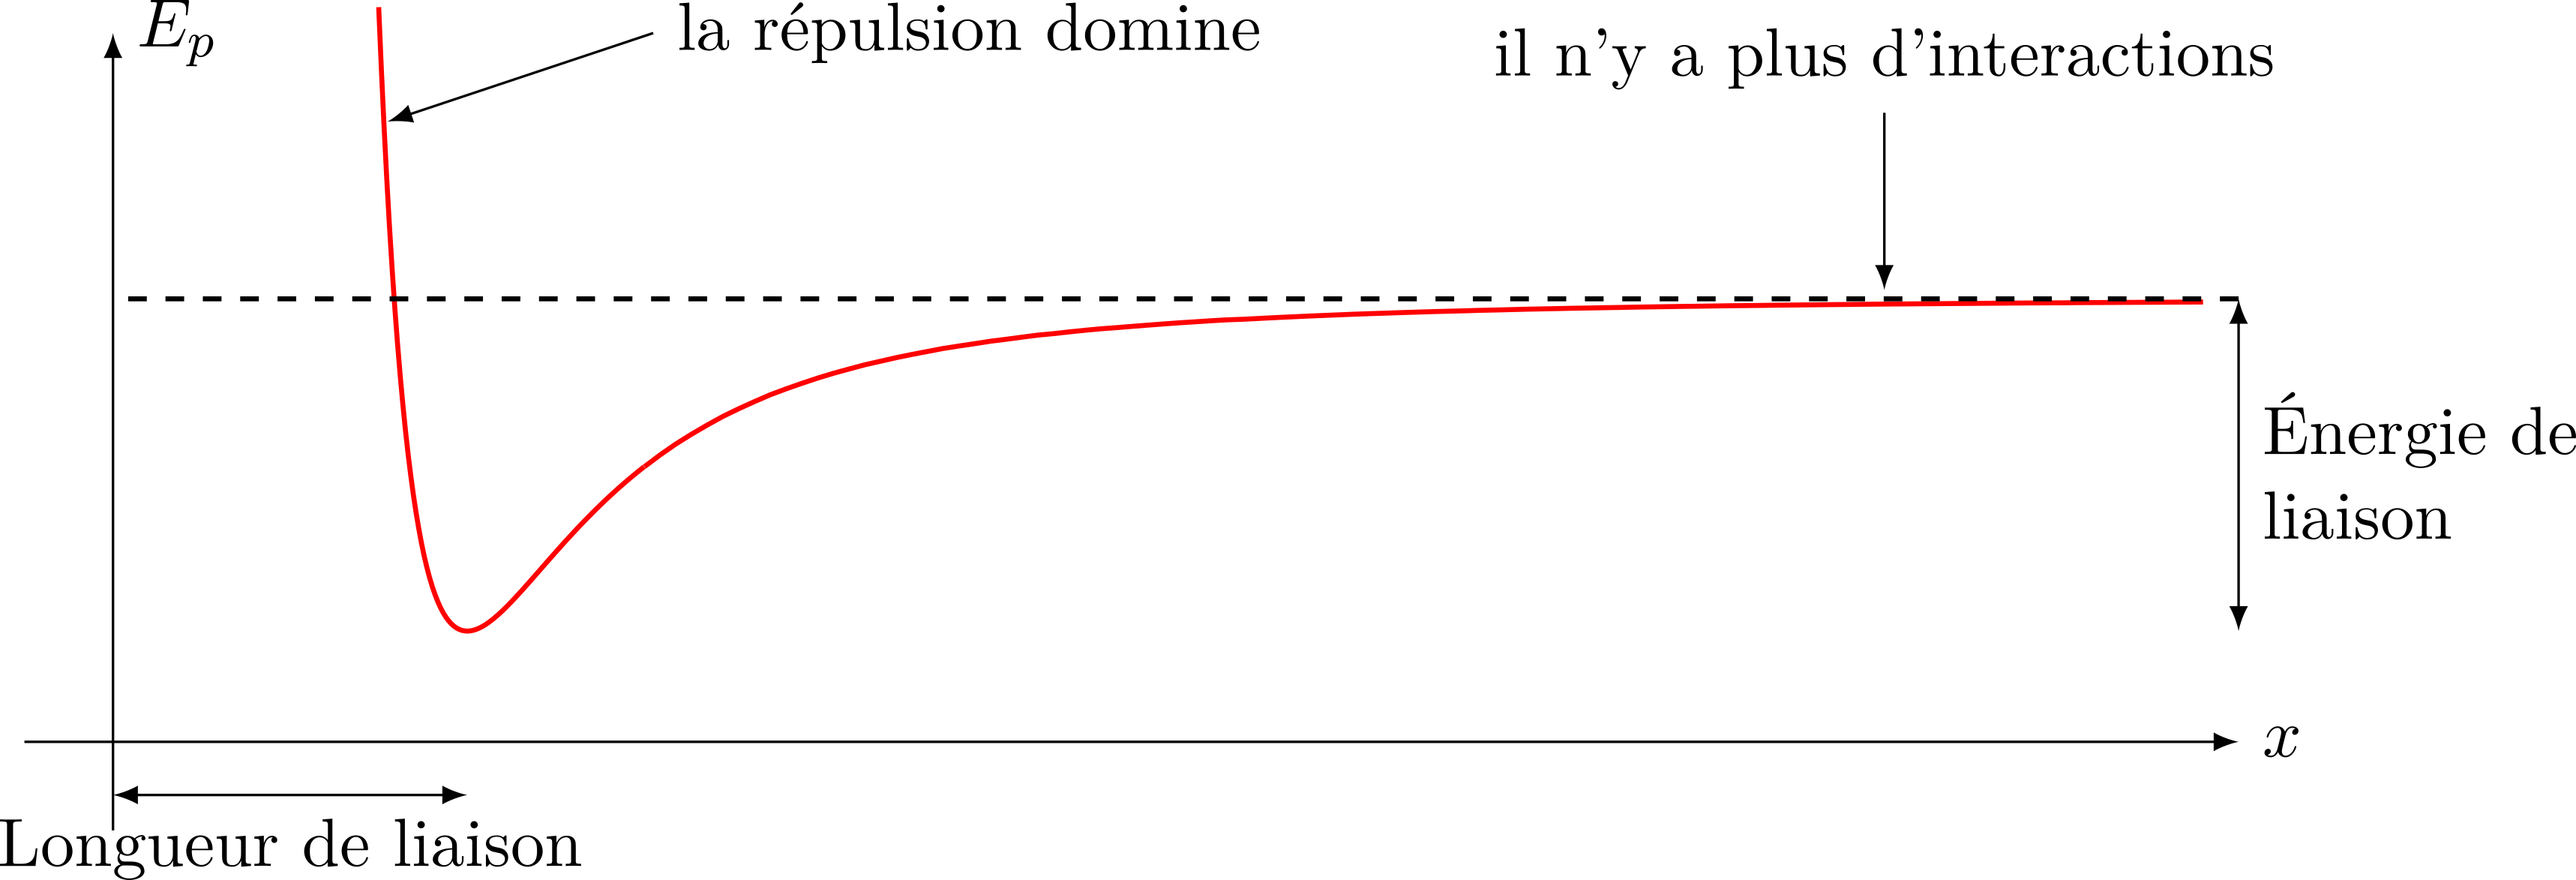
\includegraphics[scale=1]{lgcov}
	}
	\caption{Énergie potentielle totale entre un atome considéré fixe à $x=0$ et
		un autre atome s'en approchant. On a d'abord une attraction noyau/noyau à
		grande distance qui les attirent, puis leurs nuages électroniques se
		repoussent à faible distance. Le puits de potentiel correspond à l'équilibre
		mécanique de cette interaction, et la hauteur depuis le fond du puits
		jusqu'à l'absence d'interaction correspond à l'énergie de la liaison, i.e.\
		l'énergie à fournir pour séparer les deux atomes ainsi liés.}
	\label{fig:lgcov}
\end{figure}

L'ordre de grandeur de la longueur de la liaison est de \textbf{\SI{100}{pm}},
et l'énergie de la liaison de \textbf{$\SI{500}{kJ.mol^{-1}}$}~; elle correspond
à l'énergie à fournir pour rompre toutes les liaisons d'une \textit{mole} de la
molécule considérée sous forme \textit{gazeuse}. Les liaisons doubles sont plus
courtes et plus intenses que les simples.

\begin{table}[ht]
	\centering
	\caption{Exemples de liaisons, longueur et énergies.}
	\label{tab:covalue}
	\begin{tabular}{lccccccccc}
		\toprule
		Liaison                      &
		\ce{C-H}                     & \ce{C-C} & \ce{C-N} & \ce{C-O} & \ce{C-F} & \ce{C-Cl} & \ce{C=C}
		                             & \ce{C=O}
		\\\midrule
		Longueur (\si{pm})           &
		109                          & 154      & 147      & 143      & 135      & 177       & 134      & 120
		\\\midrule
		Énergie ($\si{kJ.mol^{-1}}$) &
		415                          & 347      & 305      & 356      & 439      & 327       & 615      & 743
		\\\bottomrule
	\end{tabular}
\end{table}

\subsubsection{Règle du duet et de l'octet}
Un atome de couche de valence pleine est stable. Lors de la formation de
liaisons avec d'autres atomes, ils vont s'associer pour compléter ces couches.
On a ainsi~:

\begin{tcb*}(ror){Règle de l'octet et du duet}
	Les atomes formes des molécules dans lesquels leur stabilité est accrue, en
	complétant leur couche de valence. Ainsi, ils sont entourés de~:
	\begin{tasks}(2)
		\task \psw{
			1 doublet  (2 électrons) pour l'hydrogène~;
		}
		\task \psw{
			4 doublets (8 électrons) pour les autres.
		}
	\end{tasks}
\end{tcb*}

\subsection{Notation de \textsc{Lewis} des molécules}
\subsubsection{Présentation}

\begin{tcb*}(defi){Représentation de \textsc{Lewis} d'une molécule}
	\psw{
		Le schéma de \textsc{Lewis} d'une molécule ou d'un ion polyatomique
		représente les atomes de à plat  avec \textbf{tous leurs électrons de
			valence}. Un \textbf{tiret} représente un \textbf{doublet}, qui peut être
		\textbf{non-liant} si localisé sur un atome, et \textbf{liant} s'il est
		partagé entre deux atomes.
	}
\end{tcb*}

\begin{table}[ht]
	\centering
	\caption{Représentations de \textsc{Lewis} de molécules}
	\begin{tabular}{lP{4cm}lP{4cm}}
		\toprule
		Eau~\ce{H2O}
		 &
		\psw{
			\cfig{\lewis{13,O}
				(-[7,.7]H)
				(-[5,.7]H)
			}
		}
		 &
		Méthane~\ce{CH4}~:
		\psw{
		\cfig{C
		(-[0,.5]H)
		(-[2,.5]H)
		(-[4,.5]H)
		(-[6,.5]H)
		}
		}
		\\[1em]
		Diazote~\ce{N2}~:
		 &
		\psw{
			\cfig{\lewis{4,N}~\lewis{0,N}}
		}
		 &
		Dioxygène~\ce{O2}~:
		\psw{
			\cfig{\lewis{35,O}=\lewis{17,O}}
		}
		\\
		\bottomrule
	\end{tabular}
	\label{tab:lewismol}
\end{table}

\subsubsection{Charge formelle}
Lors de la formation de liaisons covalentes, il peut y avoir une perte ou gain
d'électrons par rapport à l'atome neutre, représenté par une \textbf{charge
	formelle} localisée sur l'atome en question dans le schéma de \textsc{Lewis}.

\begin{tcb*}(exem)<lftt>'l'{Charge formelle}
	\begin{minipage}[t]{0.48\linewidth}
		Charge formelle $\ominus$ sur l'oxygène dans \ce{HO-}~:
		\vspace{1cm}
		\psw{
			\[
				\cfig{H-\chemabove{\lewis{602,O}}{\hspace{20pt}\ominus}}
			\]
		}
	\end{minipage}
	\hfill
	\begin{minipage}[t]{0.48\linewidth}
		Charge formelle $\oplus$ sur l'azote dans \ce{NH4+}~:
		\psw{
			\[
				\cfig{
					\chemabove{N}{\hspace{20pt}\oplus}
					(-[0,.7]H)
					(-[2,.7]H)
					(-[4,.7]H)
					(-[6,.7]H)
				}
			\]
		}
		\vspace{-15pt}
	\end{minipage}
\end{tcb*}

\begin{tcb*}(tool){Charge formelle}
	Pour établir cette charge formelle, on compte le nombre d'électrons qui
	entourent directement l'atome dans le schéma de \textsc{Lewis}~:
	\begin{itemize}
		\item \psw{
			      Les \textbf{doublets non-liants} comptent pour \textbf{2 électrons}~;
		      }
		\item \psw{
			      Les \textbf{doublets liants} comptent pour \textbf{1 électron}
			      puisqu'il se partage entre les deux atomes.
		      }
	\end{itemize}
	On en déduit la charge formelle avec la formule
	\psw{
		\[\boxed{C = V - L}\]
	}
	avec $C$ la charge formelle, $V$ son nombre d'électrons de valence dans l'état
	neutre, $L$ le nombre d'électrons qui l'entourent dans la molécule.
\end{tcb*}

Ainsi, dans l'ion \ce{HO-}, l'oxygène est entouré de $3*2+1=7$ électrons contre
6 dans son état isolé, c'est 1 de plus que son état de valence sous forme
d'atome neutre~: il porte donc une charge $\ominus$. Pour l'azote c'est
l'inverse~: il est ici entouré de $4*1=4$ électrons, contre 5 dans son état
isolé, c'est un de moins que son état de valence sous forme neutre et il porte
donc une charge $\oplus$.

\begin{tcb*}(impo){Règle de l'octet vs.\ charge formelle}
	La règle de l'octet et la charge formelle ne fonctionnent pas de la même
	manière~: pour respecter la règle de l'octet un atome s'entoure de \textbf{4
		doublets} qui représentent donc 8 électrons, mais dans le décompte des
	électrons qui gravitent autour de lui on compte les électrons les plus
	proches, donc un doublet liant est 1 seul électron.
\end{tcb*}

\begin{tcb*}[breakable](appl)<lftt>'l'{Charges formelles}
	Placer les charges formelles sur les structures suivantes~:
	\[
		\cfig{\lewis{4,C}~\lewis{0,N}}
		\qquad\qquad
		\cfig{
		C
		(-[0,.7]\lewis{602,O})
		(-[4,.7]\lewis{246,O})
		(=[6,.7]\lewis{57,O})
		}
	\]
	\tcblower
	\begin{enumerate}
		\item \psw{
			      Pour l'ion cyanure \ce{CN-}~:
			      \begin{itemize}
				      \item L'azote compte 3 DL et 1 DnL, soit $3*1+2=5$ électrons. Il
				            a normalement 5 électrons de valence, donc $C(\ce{N}) =
					            0$.
				      \item Le carbone a également 3DL et 1DnL, soit 5 électrons. Il a
				            normalement 4 électrons de valence, d'où $C(\ce{C}) = 4-5
					            = -1$ et il porte une charge $\ominus$.
			      \end{itemize}
			      \[
				      \cfig{\chemabove{\lewis{4,C}}{\hspace{-20pt}\ominus}~\lewis{0,N}}
			      \]
		      }
		      \vspace{-15pt}
		\item \psw{
		      Pour l'ion carbonate \ce{CO3^{2-}}~:
		      \begin{itemize}
			      \item Le carbone a 4DL donc 4 électrons, donc pas de charge.
			      \item L'oxygène du bas a 2DnL et 2DL, donc $2*2+2*1=6$
			            électrons, égal à son nombre d'électrons de valence, donc
			            pas de charge.
			      \item Les oxygènes de gauche et de droite ont 3DnL et 1DL soit
			            $3*2+1*1=7$ électrons, d'où $C(O) = 6-7 = -1$ et ils
			            portent chacun une charge $\ominus$
		      \end{itemize}
		      \[
			      \cfig{
			      C
			      (-[0,.7]\chemabove{\lewis{602,O}}{\hspace{-20pt}\ominus})
			      (-[4,.7]\chemabove{\lewis{246,O}}{\hspace{-20pt}\ominus})
			      (=[6,.7]\lewis{57,O})
			      }
		      \]
		      }
		      \vspace{-15pt}
	\end{enumerate}
\end{tcb*}

\subsubsection{Bilan des structures possibles}
\begin{itemize}[label=$\diamond$]
	\item Pour l'hydrogène~: un seul doublet, nécessairement liant pour une
	      molécule, sinon ion monoatomique \ce{H+}~:
	      \vspace*{-10pt}
	      \psw{
		      \begin{center}
			      \hfill
			      \cfig{H-}
			      \hfill
			      \cfig{\chemabove{\lewis{4|,H}}{\hspace{20pt}\oplus}}
			      \hfill~
		      \end{center}
	      }
	\item Pour le carbone~: quatre doublets liants et pas de charge, ou un DnL
	      et trois DL donc une charge $\ominus$~:
	      \vspace*{-10pt}
	      \psw{
		      \begin{center}
			      \hfill
			      \cfig{C(-[0,.7])(-[2,.7])(-[4,.7])(-[6,.7])}
			      \hfill
			      \cfig{
				      \chemabove{\lewis{2,C}}{\hspace{20pt}\ominus}
				      (-[0,.7])(-[4,.7])(-[6,.7])
			      }
			      \hfill~
		      \end{center}
	      }
	\item Pour l'azote~: 4DL ($\oplus$), un DnL et 3 DL (0), 2DnL et 2DL
	      ($\ominus$)~:
	      \psw{
		      \begin{center}
			      \hfill
			      \cfig{
				      \chemabove{N}{\hspace{20pt}\oplus}
				      (-[0,.7])
				      (-[2,.7])
				      (-[4,.7])
				      (-[6,.7])
			      }
			      \hfill
			      \cfig{
				      \lewis{2,N}
				      (-[0,.7])(-[4,.7])(-[6,.7])
			      }
			      \hfill
			      \cfig{-\chemabove{\lewis{26,N}}{\hspace{20pt}\ominus}-}
			      \hfill~
		      \end{center}
	      }
	\item Pour l'oxygène~: 1DnL et 3DL ($\oplus$), 2DnL et 2DL (0), 3DnL et 1DL
	      ($\ominus$)~:
	      \psw{
		      \begin{center}
			      \hfill
			      \cfig{
				      \chemabove{\lewis{2,O}}{\hspace{20pt}\oplus}
				      (-[0,.7])(-[4,.7])(-[6,.7])
			      }
			      \hfill
			      \cfig{-\lewis{26,O}-}
			      \hfill
			      \cfig{-\chemabove{\lewis{026,O}}{\hspace{20pt}\ominus}}
			      \hfill~
		      \end{center}
	      }
	\item Pour les halogènes~: 1DnL et 3DL (0), 4DnL (ion monoatomique
	      $\ominus$)~:
	      \psw{
		      \begin{center}
			      \hfill
			      \cfig{-\lewis{026,Cl}}
			      \hfill
			      \cfig{\chemabove{\lewis{0246,Cl}}{\hspace{20pt}\ominus}}
			      \hfill~
		      \end{center}
	      }
\end{itemize}

\vspace{-15pt}
\subsubsection{Obtention d'une représentation de \textsc{Lewis}}
\begin{tcb*}(tool){Méthode pour déterminer une représentation de \textsc{Lewis}}
	\begin{enumerate}[label=\sqenumi]
		\bitem{Compter} le nombre total d'électrons de valence \textbf{sans oublier
			les charges formelles}, en déduire le nombre
		de doublets à placer~;
		\bitem{Assembler} les atomes entre eux, en plaçant de préférence les atomes
		faisant le plus de liaisons au centre~;
		\bitem{Placer} les doublets de façon à respecter l'octet~: on peut commencer
		par les DL simples et combler le reste avec des DnL, s'il y a trop de
		DnL on aura une liaison multiple~;
		\bitem{Ajouter} les charges formelles~;
		\bitem{Vérifier} que chaque atome est entouré de 4 doublets, qu'il y a le
		bon nombre de doublet total, et que la charge totale est bonne.
	\end{enumerate}
\end{tcb*}

\begin{tcb*}[breakable](appl)<lftt>'l'{Représentations de \textsc{Lewis}}
	\begin{enumerate}
		\bitem{Méthanal \ce{CH2O}}~:
		\begin{itemize}[label=$\triangleright$, leftmargin=20pt]
			\item Décompte des électrons~:
			      \begin{itemize}[label=$\ra$, leftmargin=20pt]
				      \item $[\ce{H}]~:$
				            \psw{
					            $\lsw{red}{\rm 1s^{1}}$ donc 1 électron de valence
				            }
				      \item $[\ce{C}]~:$
				            \psw{
					            $\rm 1s^2\lsw{red}{2s^22p^2}$ donc 4 électrons de valence
				            }
				      \item $[\ce{O}]~:$
				            \psw{
					            $\rm 1s^2\lsw{red}{2s^22p^4}$ donc 6 électrons de valence.
				            }
				      \item Total~:
				            \psw{
					            $2*1 + 4 + 6 = 12$ électrons, 6 doublets.
				            }
			      \end{itemize}
			\item Méthode simple~:
			      \psw{
				      on suppose le carbone central puisqu'il
				      fait le plus de connexions. On remplit ce squelette avec
				      3DL~:
				      \begin{center}
					      \cfig{
					      C
					      (-[0]O)
					      (-[3]H)
					      (-[5]H)
					      }
				      \end{center}
				      Il reste donc 3 doublets à placer. Les hydrogènes respectent
				      déjà la règle du duet. \textbf{Si tous les doublets restant
					      étaient non-liants}, il en faudrait 1 sur le carbone et 3
				      sur l'oxygène pour qu'ils respectent individuellement
				      l'octet~: c'est 1 de trop que de doublets disponibles. Il y
				      a donc une liaison double \ce{C=O}, et il reste 2DnL à
				      placer sur \ce{O}, d'où~:
				      \begin{center}
					      \cfig{
					      C
					      (=[0]\lewis{17,O})
					      (-[3]H)
					      (-[5]H)
					      }
				      \end{center}
			      }
		\end{itemize}
		\bitem{Ion cyanure \ce{CN-}}~:
		\begin{itemize}[label=$\triangleright$, leftmargin=20pt]
			\item Décompte des électrons~:
			      \psw{
				      \begin{itemize}[label=$\ra$, leftmargin=20pt]
					      \item $[\ce{C}]~: \rm 1s^2\lsw{red}{2s^22p^2}$
					            donc 4 électrons de valence
					      \item $[\ce{N}]~: \rm 1s^2\lsw{red}{2s^22p^3}$
					            donc 5 électrons de valence.
					      \item Une charge moins donc un électron en plus.
					      \item Total~: $4 + 5 + 1 = 10$ électrons, 5
					            doublets.
				      \end{itemize}
			      }
			\item Méthode simple~:
			      \psw{
				      le squelette est évident. On remplit ce squelette avec 1DL~:
				      \begin{center}
					      \cfig{
						      C-N
					      }
				      \end{center}
				      Il reste donc 4 doublets à placer. \textbf{Si tous les
					      doublets restant étaient non-liants}, il en faudrait 3 sur
				      le carbone et 3 sur l'azote pour qu'ils respectent
				      individuellement l'octet~: c'est 2 de trop que de doublets
				      disponibles. Il y a donc une liaison triple \ce{C#N}, et il
				      reste 2DnL à placer sur \ce{C} et sur \ce{N}, d'où~:
				      \begin{center}
					      \cfig{
						      \lewis{4,C}~\lewis{0,N}
					      }
				      \end{center}
			      }
			\item Charges formelles~:
			      \psw{
				      déjà fait plus tôt, \ce{C} porte une charge $\ominus$.
				      \begin{center}
					      \cfig{\chemabove{\lewis{4,C}}{\hspace{-20pt}\ominus}~\lewis{0,N}}
				      \end{center}
			      }
		\end{itemize}
		\bitem{Ion nitrate \ce{NO3-}}~:
		\begin{itemize}[label=$\triangleright$, leftmargin=20pt]
			\item Décompte des électrons~:
			      \psw{
				      \begin{itemize}[label=$\ra$, leftmargin=20pt]
					      \item $[\ce{N}]~: \rm 1s^2\lsw{red}{2s^22p^3}$
					            donc 5 électrons de valence.
					      \item $[\ce{O}]~: \rm 1s^2\lsw{red}{2s^22p^4}$
					            donc 6 électrons de valence.
					      \item Une charge moins donc un électron en plus.
					      \item Total~: $5 + 3*6 + 1 = 24$ électrons, 12
					            doublets.
				      \end{itemize}
			      }
			\item Méthode simple~:
			      \psw{
				      on suppose l'azote central puisqu'il
				      fait le plus de connexions. On remplit ce squelette avec
				      3DL~:
				      \begin{center}
					      \cfig{
					      N
					      (-[0]O)
					      (-[4]O)
					      (-[6]O)
					      }
				      \end{center}
			      }
			      \psw{
				      Il reste donc 9 doublets à placer. \textbf{Si tous les
					      doublets restant étaient non-liants}, il en faudrait 1 sur
				      l'azote et 3 sur chaque oxygène pour qu'ils respectent
				      individuellement l'octet~: c'est 1 de plus que de doublets
				      disponibles. Il y a donc une liaison double \ce{N=O}, et il
				      reste 8DnL à placer sur les \ce{O} restant puisque l'azote
				      vérifie déjà l'octet, d'où~:
				      \begin{center}
					      \cfig{
					      N
					      (-[0]\lewis{602,O})
					      (-[4]\lewis{246,O})
					      (=[6]\lewis{57,O})
					      }
				      \end{center}
			      }
			\item Charges formelles~:
			      \psw{
				      cf.\ plus tôt, \ce{N} porte une
				      charge $\oplus$ et les \ce{O} de gauche et droite portent
				      une charge $\ominus$, pour une charge totale effectivement
				      égale à $-e$.
				      \begin{center}
					      \cfig{
						      \chemabove{N}{\hspace{20pt}\oplus}
						      (-[0]\chemabove{\lewis{602,O}}{\hspace{20pt}\ominus})
						      (-[4]\chemabove{\lewis{246,O}}{\hspace{-20pt}\ominus})
						      (=[6]\lewis{57,O})
					      }
				      \end{center}
			      }
		\end{itemize}
	\end{enumerate}
\end{tcb*}

\subsection{Écarts à la règle de l'octet}
Il faut être capable d'identifier les écarts cités, mais il ne faut pas les
connaître par cœur.

\subsubsection{Composés électrodéficients}
\begin{tcb*}(defi){Électrodéficience}
	Un atome ne pouvant pas s'entourer d'un doublet d'électrons est dit
	\textbf{électrodéficient}. Deux cas se présentent~:
	\smallbreak
	\begin{isd}[sidebyside align=top]
		\tcbsubtitle{\fatbox{\textbf{Composés lacunaires}}}
		\psw{
			S'il lui en manque un nombre pair, on le représente par une
			\textbf{lacune}, traduisant une OA vide.
		}
		\tcblower
		\tcbsubtitle{\fatbox{\textbf{Composés radicaux}}}
		\psw{
			S'il lui en manque un nombre impair, on le représente par des
			\textbf{électrons célibataires}.
		}
	\end{isd}
\end{tcb*}

\begin{tcb*}(exem)<lftt>{Composés électrodéficients}
	\psw{
		\begin{center}
			\hfill
			\cfig{
				\lewis{2|,Al}
				(-[0]\lewis{602,Cl})
				(-[4]\lewis{246,Cl})
				(-[6]\lewis{046,Cl})
			}
			\hfill
			\cfig{H-\lewis{2|6|,Be}-H}
			\hfill
			\cfig{\lewis{35,O}=\lewis{2,N}-\lewis{6.02,O}}
			\hfill~
		\end{center}
	}
	\vspace{-15pt}
\end{tcb*}

\subsubsection{Hypervalents}

\begin{tcb*}(defi){Hypervalence}
	Lorsqu'un atome s'entoure de plus de 4 doublets d'électrons, on dit qu'il
	est \textbf{hypervalent}. Cette situation n'est possible qu'\textbf{à partir
		de la 3ème période} (OA d font des liaisons).
\end{tcb*}

\begin{tcb*}(exem)<lftt>'l'{Composés hypervalents}
	\psw{
		\begin{center}
			\hfill
			\cfig{
			P
			(-[0]\lewis{026,Cl})
			(-[2]\lewis{024,Cl})
			(-[3]\lewis{246,Cl})
			(-[5]\lewis{246,Cl})
			(-[6]\lewis{046,Cl})
			}
			\hfill
			\cfig{
			S
			(-[0]\chemabove{\lewis{602,O}}{\hspace{20pt}\ominus})
			(=[2]\lewis{13,O})
			(-[4]\chemabove{\lewis{246,O}}{\hspace{-20pt}\ominus})
			(=[6]\lewis{57,O})
			}
			\hfill~
		\end{center}
	}
	\vspace{-15pt}
\end{tcb*}

\subsubsection{Bilan}

\begin{table}[H]
	\centering
	\caption{Possibilités d'interactions covalentes selon la période.}
	\label{tab:oclachy}
	\begin{tabular}{lcc}
		\toprule
		Caractéristique       &
		2\ieme\ période       &
		3\ieme\ période
		\\\midrule
		Octet~: 8 é.          & Systématique       & Très souvent
		\\
		Lacune~: < 8 é.       & Rare mais possible & Rare mais possible
		\\
		Hypervalence~: > 8 é. & Impossible         & Souvent
		\\\bottomrule
	\end{tabular}
\end{table}

\subsection{Limite du modèle de \textsc{Lewis}}
\begin{itemize}
	\item Dans les cristaux, on observe un ordre à longue distance. La cohésion
	      est assurée par différentes interactions dépendant des cristaux (forces
	      intermoléculaires, liaison métallique, liaison ionique). Dans ces cas,
	      le modèle de \textbf{Lewis} n'est pas pertinent pour décrire leur
	      structure.
	\item Le modèle de \textbf{Lewis} ne permet pas de connaître la géométrie
	      des molécules, alors que celle-ci a beaucoup d'implications sur la
	      chimie.
	\item Certaines propriétés, notamment magnétiques, ne peuvent pas être
	      expliquées par ce modèle.
	\item Il existe également des liaisons intermédiaires entre la liaison
	      double et la liaison simple : la réalité est une «~moyenne~» entre deux
	      représentations de \textbf{Lewis}.
\end{itemize}

\begin{tcb*}(exem)<lftt>'l'{Limites au modèle de \textsc{Lewis}}
	Les trois représentations de \textsc{Lewis} ci-dessous sont possibles, et
	coexistent~:
	\begin{center}
		\hfill
		\cfig{
			\chemabove{N}{\hspace{20pt}\oplus}
			(-[0]\chemabove{\lewis{602,O}}{\hspace{20pt}\ominus})
			(=[4]\lewis{35,O})
			(-[6]\chemabove{\lewis{460,O}}{\hspace{-20pt}\ominus})
		}
		\hfill
		\cfig{
			\chemabove{N}{\hspace{20pt}\oplus}
			(-[0]\chemabove{\lewis{602,O}}{\hspace{20pt}\ominus})
			(-[4]\chemabove{\lewis{246,O}}{\hspace{-20pt}\ominus})
			(=[6]\lewis{57,O})
		}
		\hfill
		\cfig{
			\chemabove{N}{\hspace{20pt}\oplus}
			(=[0]\lewis{71,O})
			(-[4]\chemabove{\lewis{246,O}}{\hspace{-20pt}\ominus})
			(-[6]\chemabove{\lewis{460,O}}{\hspace{-20pt}\ominus})
		}
		\hfill~
	\end{center}
	et la réalité est une moyenne des trois (notamment, chaque liaison est de
	longueur égale à la moyenne pondérée des liaisons \ce{C-O} et \ce{C=O}).
	C'est également la cas pour l'ozone~:
	\begin{center}
		\hfill
		\cfig{\lewis{35,O}=
			\chemabove{\lewis{2,O}}{\vspace{10pt}\hspace{20pt}\oplus}
			-\chemabove{\lewis{026,O}}{\vspace{-12pt}\hspace{20pt}\ominus}
		}
		\hfill
		\cfig{
			\chemabove{\lewis{246,O}}{\vspace{-12pt}\hspace{-20pt}\ominus}-
			\chemabove{\lewis{2,O}}{\vspace{10pt}\hspace{20pt}\oplus}=
			\lewis{17,O}
		}
		\hfill~
	\end{center}
\end{tcb*}

\section{Géométrie et polarité des entités chimiques}
\subsection{Géométrie~: modèle VSEPR}
\subsubsection{Introduction}

La répartition des atomes d'une molécule dans l'espace est une donnée précieuse.
On observe une certaine diversité dans les agencement spatiaux qui fait partie
de la diversité des interactions moléculaires~:
\begin{center}
	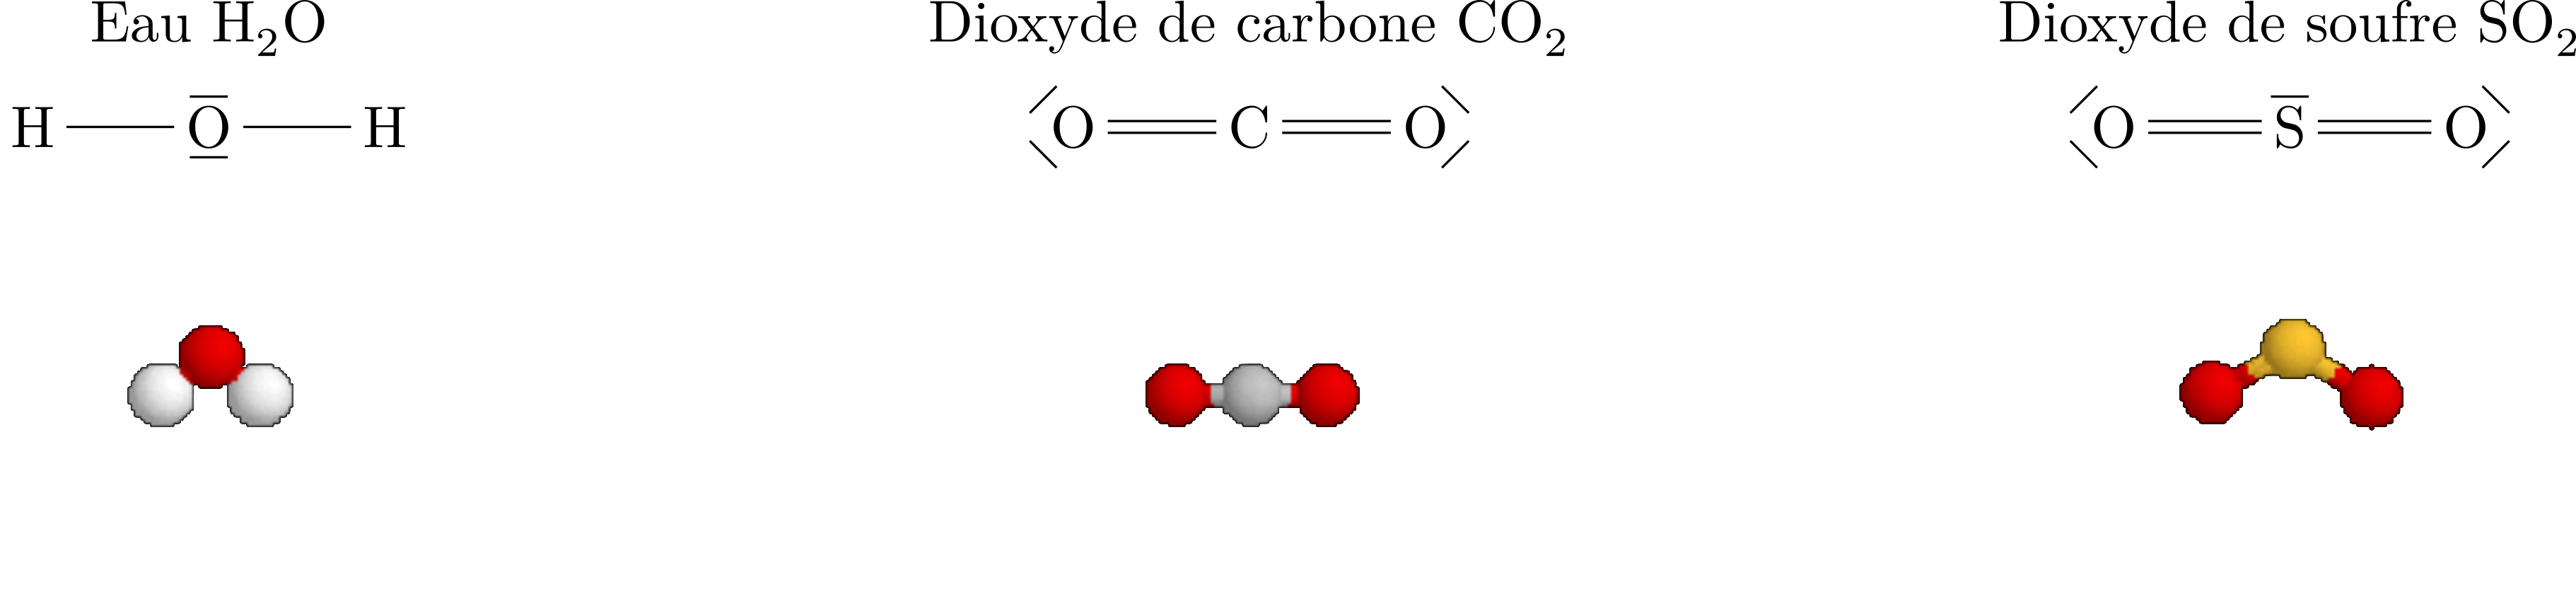
\includegraphics[scale=1]{introvsepr_a-white}
\end{center}
\begin{center}
	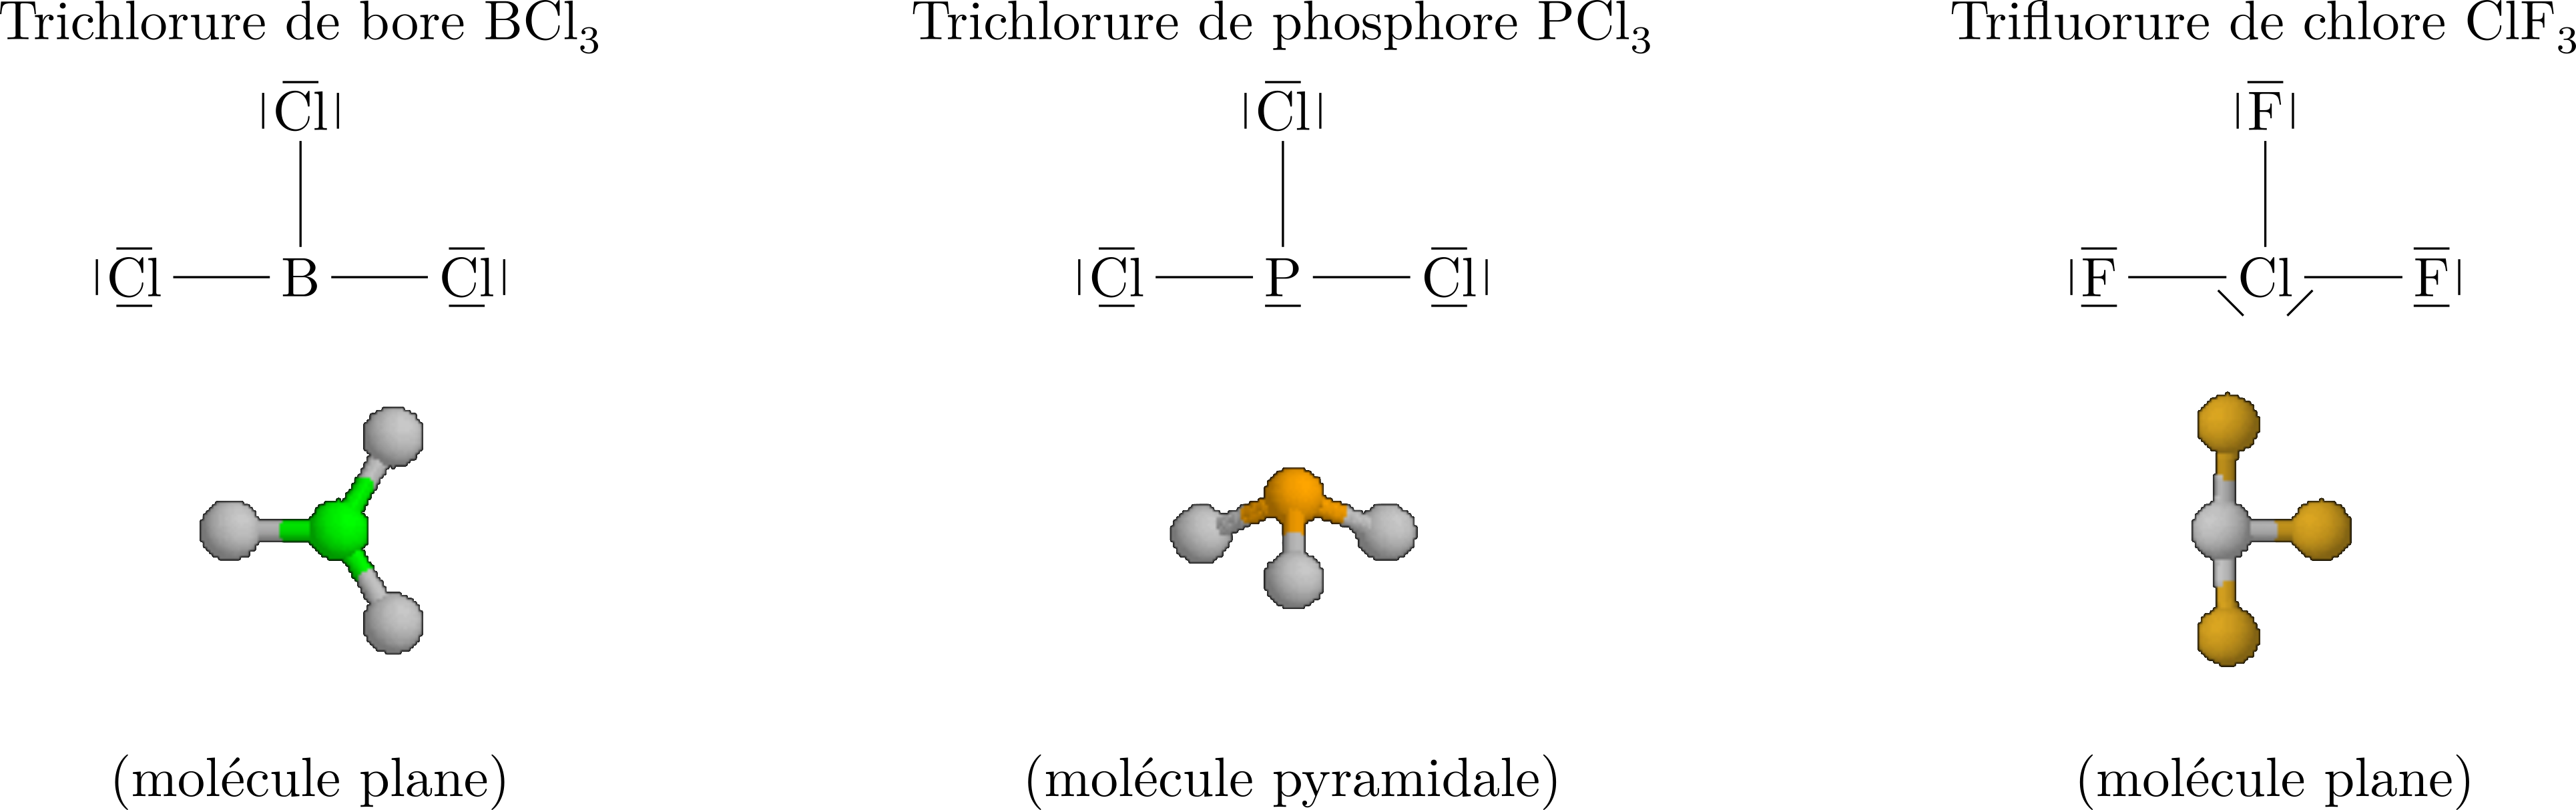
\includegraphics[scale=1]{introvsepr_b-white}
\end{center}
De ces exemples, on peut formuler trois observations~:
\begin{enumerate}
	\item \psw{
		      Le schéma de \textsc{Lewis} ne donne \textbf{aucune information sur la
			      géométrie de la molécule}~: des molécules dont les schémas de
		      \textsc{Lewis} se ressemblent peuvent avoir des géométries différentes.
	      }
	\item \psw{
		      Il semble que l'atome central ait un rôle prépondérant par rapport aux
		      atomes latéraux.
	      }
	\item \psw{
		      La géométrie semble fortement conditionnée par l'existence de doublets
		      non liants autour de l'atome central.
	      }
\end{enumerate}

\begin{tcb*}[cnt, bld](ror){Géométrie d'une molécule}
	\psw{
		La géométrie d'une molécule est celle qui minimise les forces de
		répulsion entre doublets d'électrons, c'est-à-dire celle pour laquelle
		les distances entre doublets sont maximales.
	}
\end{tcb*}

La régularité géométrique dans ces édifices est alors décrite par un modèle, le
modèle VSEPR pour \textit{Valence Shell Pair Electron Repulsion}\footnote{Soit
	«~Répulsion des paires d'électrons de valence~».}

\subsubsection{Représentation de \textsc{Cram}}
Pour représenter les molécules dans l'espace, on introduit une nouvelle
représentation~:
\begin{tcb*}[breakable](defi){Représentation de \textsc{Cram}}
	Dans la représentation de \textsc{Cram}, on représente une liaison simple de
	3 manières différentes selon sa disposition dans l'espace~:
	\begin{itemize}
		\item \psw{
			      Une liaison \textbf{dans le plan} est encore représentée par un
			      trait simple~;
			      \begin{center}
				      \cfig{C-C}
			      \end{center}
		      }
		\item \psw{
			      Une liaison \textbf{en avant} du plan («~sortant du tableau~») est
			      représentée par un \textbf{triangle creux (ou plein)} dont la base
			      représente l'atome le plus proche~:
			      \begin{center}
				      \hfill
				      \cfig{C>C}
				      \hfill
				      \qou
				      \hfill
				      \cfig{C>|C}
				      \hfill~
			      \end{center}
		      }
		\item \psw{
			      Une liaison \textbf{en arrière} du plan («~rentrant dans le
			      tableau~») est représentée par un \textbf{triangle hachuré} dont la
			      base représente l'atome le plus loin~:
			      \begin{center}
				      \cfig{C>:C}
			      \end{center}
		      }
	\end{itemize}
\end{tcb*}

\begin{tcb*}(exem)<lftt>'l'{Représentations de \textsc{Cram}}
	Le méthane \ce{CH4} organise ses atomes dans l'espace de la manière
	suivante~:
	\begin{center}
		\cfig{C(-[2,.7]H)(<:[5]H)(<[6]H)(-[7]H)}
	\end{center}
	Ici, les deux liaisons \ce{C-H} identiques sont dans le plan de la feuille,
	alors que la \ce{C-H} du bas est dirigée vers nous et celle de gauche
	dirigée à l'opposé de nous. Cette structure est celle d'une pyramide à base
	triangulaire, nous le reverrons.
\end{tcb*}

\subsubsection{Modèle VSEPR}
Le modèle VSEPR repose sur l'utilisation des doublets liants \textbf{et}
non-liants pour déterminer la répartition des liaisons dans l'espace. En effet,
par leur localité,
\begin{tcb*}[cnt, bld](prop){Répulsion dues aux doublets}
	Les doublets non-liants sont plus répulsifs que les doublets liants.
\end{tcb*}

Ainsi, on étudie précisément la géométrie autour d'un atome A
lié à $n$ atomes X et porteur de $p$ doublets non-liants~; on note alors cette
géométrie \ce{AX_nE_p}.

La géométrie sera toujours donnée dans l'énoncé en français~; la signification
de l'écrite \ce{AX_nE_p} n'est \textbf{pas à connaître}, mais vous devez
connaître leur \textbf{nom et leur géométrie}. Quelques exemples pour la
culture~:
% TODO: Faire comme Lauren~!

\begin{itemize}[label=$\diamond$]
	\bitem{Linéaire} \ce{AX2}~: l'atome central a deux voisins et aucun
	doublet non-liant, comme par exemple le dioxyde de carbone \ce{CO2} ou
	l'hydrure de béryllium \ce{BeH2}~:
	\begin{center}
		\hfill
		$\vcenter{\hbox{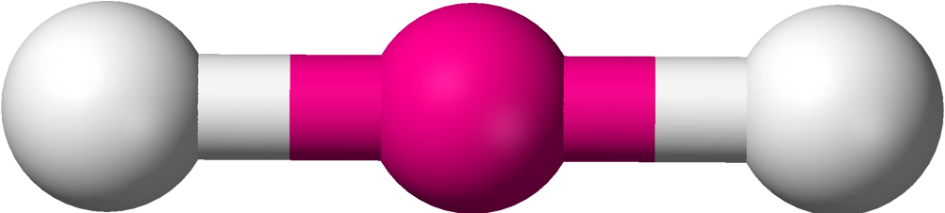
\includegraphics[scale=1]{AX2}}}$
		\hfill
		\cfig{\lewis{35,O}=C=\lewis{71,O}}
		\hfill
		\cfig{H-\lewis{2|6|,Be}-H}
		\hfill~
	\end{center}
	\bitem{Trigonale plane} \ce{AX3}~: l'atome central a trois voisins et
	aucun doublet non-liant, comme le carbocation \ce{CH3+} ou l'hydrure de bore
	\ce{BH3}. L'angle est de \ang{120} entre chaque liaison.
	\begin{center}
		\hfill
		$\vcenter{\hbox{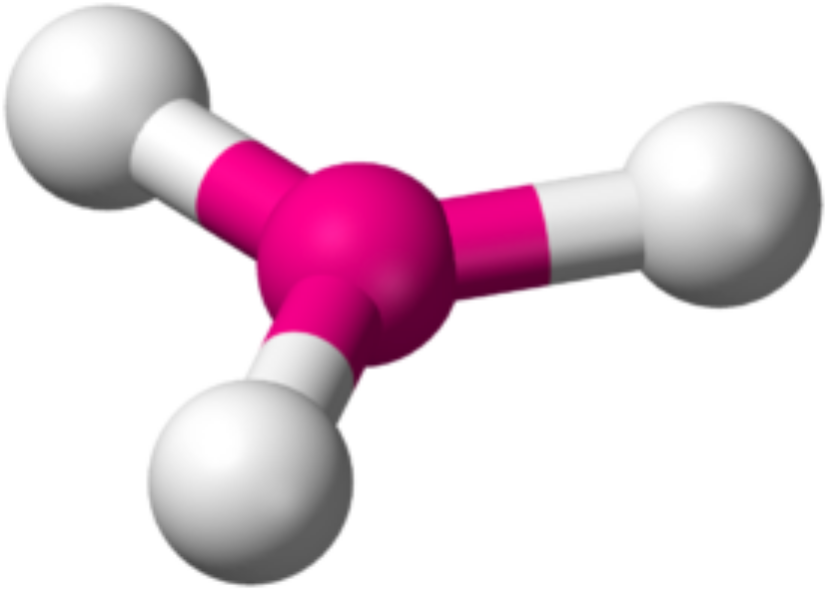
\includegraphics[scale=1]{AX3}}}$
		\hfill
		\cfig{
			\chemabove{\lewis{4|,C}}{\hspace{+20pt}\oplus}
			(-[0]H)
			(-[:120]H)
			(-[:240]H)
		}
		\hfill
		\cfig{
			\lewis{4|,B}
			(-[0]H)
			(-[:120]H)
			(-[:240]H)
		}
		\hfill~
	\end{center}
	\bitem{Coudée} \ce{AX2E1}~: 2DL 1DnL. Proche de \ce{AX3}, par exemple ozone
	\ce{O3}. L'angle est alors \textbf{inférieur à \ang{120}}.
	\begin{center}
		\hfill
		$\vcenter{\hbox{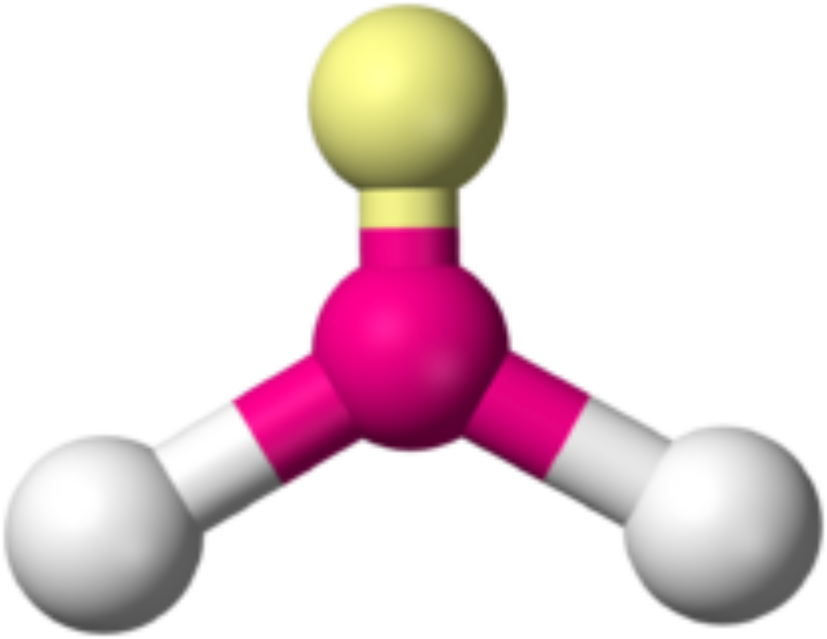
\includegraphics[scale=1]{AX2E1}}}$
		\hfill
		\cfig{
			\chemabove{\lewis{2,O}}{\hspace{-20pt}\ominus}
			(-[@{do}:-32]H)
			(-[@{go}:212]H)
		}
		\chemmove[to-to]{
			\draw
			(go) to[bend right]
			node [midway, below] {\ang{116}}
			(do)
			;}
		\hfill
		\cfig{
			\lewis{2,N}
			(-[@{dn}:-31]\chemabove{\lewis{602,O}}{\hspace{20pt}\ominus})
			(-[@{gn}:211]H)
		}
		\chemmove[to-to]{
			\draw
			(gn) to[bend right]
			node [midway, below] {\ang{118}}
			(dn)
			;}
		\hfill~
	\end{center}
	\bitem{Tétraèdrique} \ce{AX4}~: 4 voisins. Angle de
	$\arccos(-1/3)\approx\ang{109.5}$ entre chaque liaison, par exemple le
	méthane \ce{CH4}.
	\begin{center}
		\hfill
		$\vcenter{\hbox{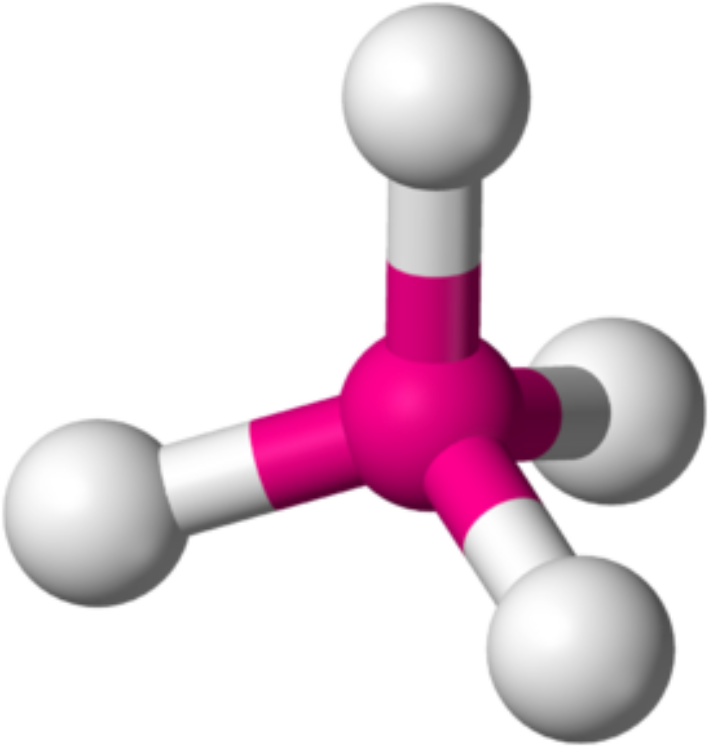
\includegraphics[scale=1]{AX4}}}$
		\hfill
		\cfig{C(-[2]H)(<:[5]H)(<[6]H)(-[7]H)}
		\hfill~
	\end{center}
	\bitem{Pyramide trigonale} \ce{AX3E1}~: 3DL, 1DnL. À cause du DnL, l'angle
	entre les DL est $<\ang{109.5}$ (\ang{107} pour l'ammoniac)~:
	\begin{center}
		\hfill
		$\vcenter{\hbox{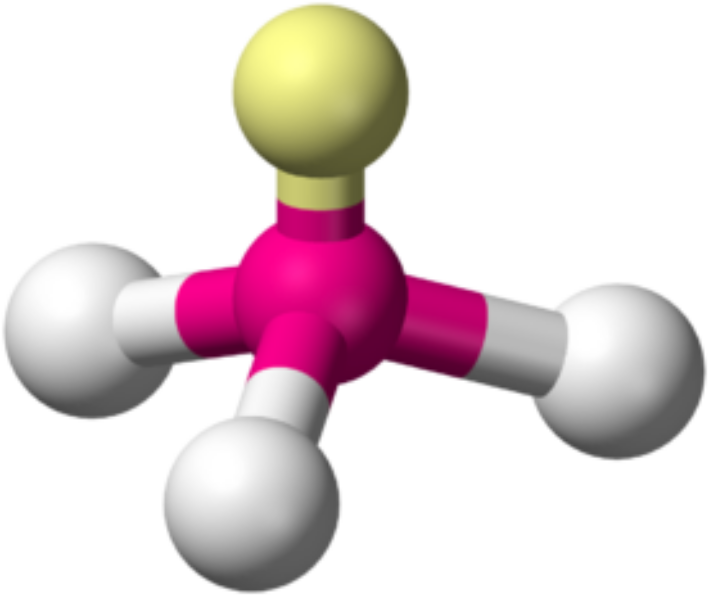
\includegraphics[scale=1]{AX3E1}}}$
		\hfill
		\cfig{\lewis{2,N}(<:[5]H)(<[6]H)(-[7]H)}
		\hfill~
	\end{center}
	\bitem{Coudée} \ce{AX2E2}~: 2DL, 2DnL. À cause des 2DnL, l'angle entre les DL
	est $<\ang{109.5}$ (\ang{104.45} pour l'eau).
	\begin{center}
		\hfill
		$\vcenter{\hbox{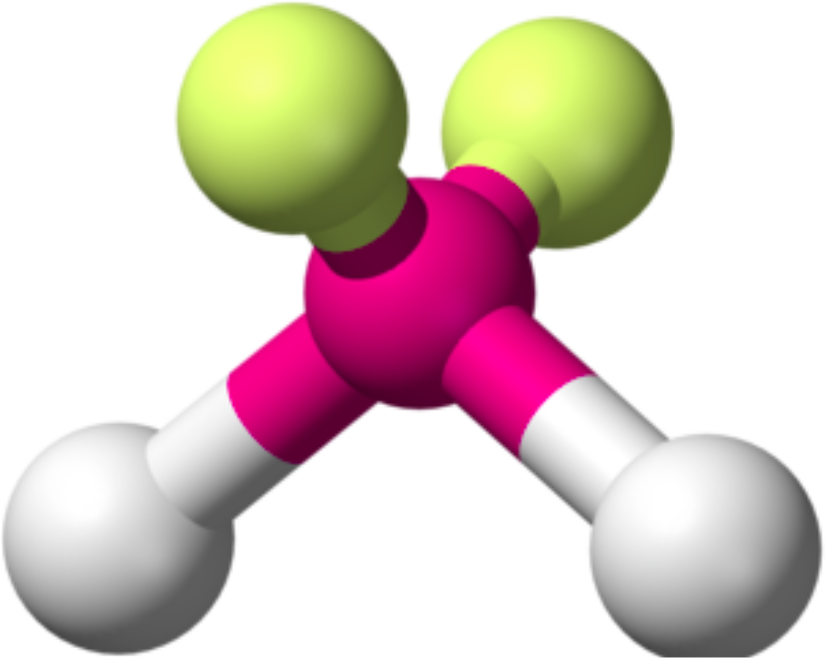
\includegraphics[scale=1]{AX2E2}}}$
		\hfill
		\cfig{
			\lewis{13,O}
			(-[@{da}:-37.775]H)
			(-[@{ga}:217.775]H)
		}
		\chemmove[to-to]{
			\draw
			(ga) to[bend right]
			node [midway, below] {\ang{104.45}}
			(da)
			;}
		\hfill~
	\end{center}
	\bitem{Bipyramide trigonale} \ce{AX5}~: 5DL, par exemple \ce{PCl5}.
	\begin{center}
		\hfill
		$\vcenter{\hbox{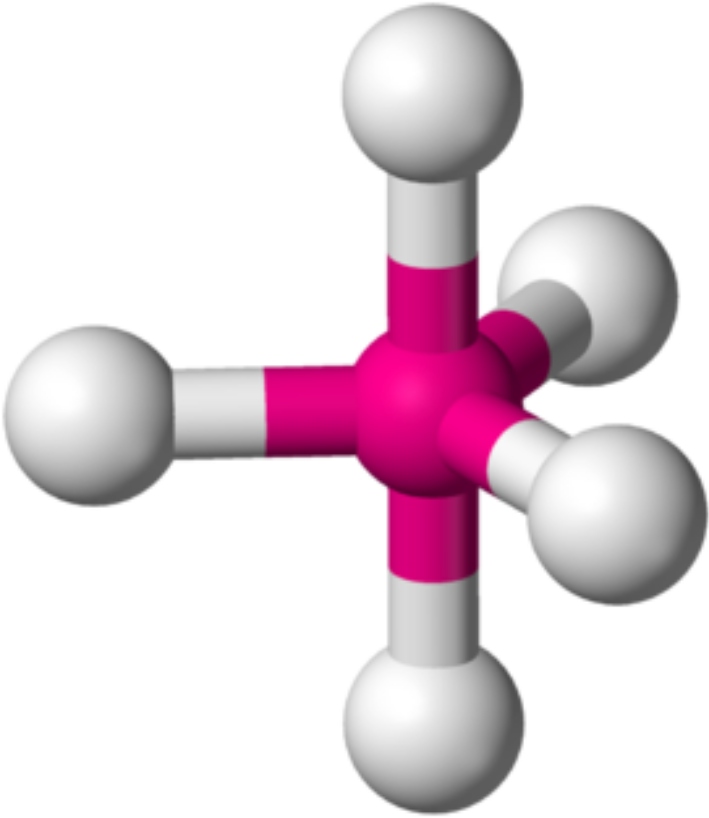
\includegraphics[scale=1]{AX5}}}$
		\hfill
		\cfig{
		P
		(-[0]\lewis{026,Cl})
		(-[2]\lewis{024,Cl})
		(<:[:150]\lewis{246,Cl})
		(<[:210]\lewis{246,Cl})
		(-[6]\lewis{046,Cl})
		}
		\hfill~
	\end{center}
	\bitem{Octaédrique}~: \ce{AX6}~: 6DL, par exemple \ce{SF6}.
	\begin{center}
		\hfill
		$\vcenter{\hbox{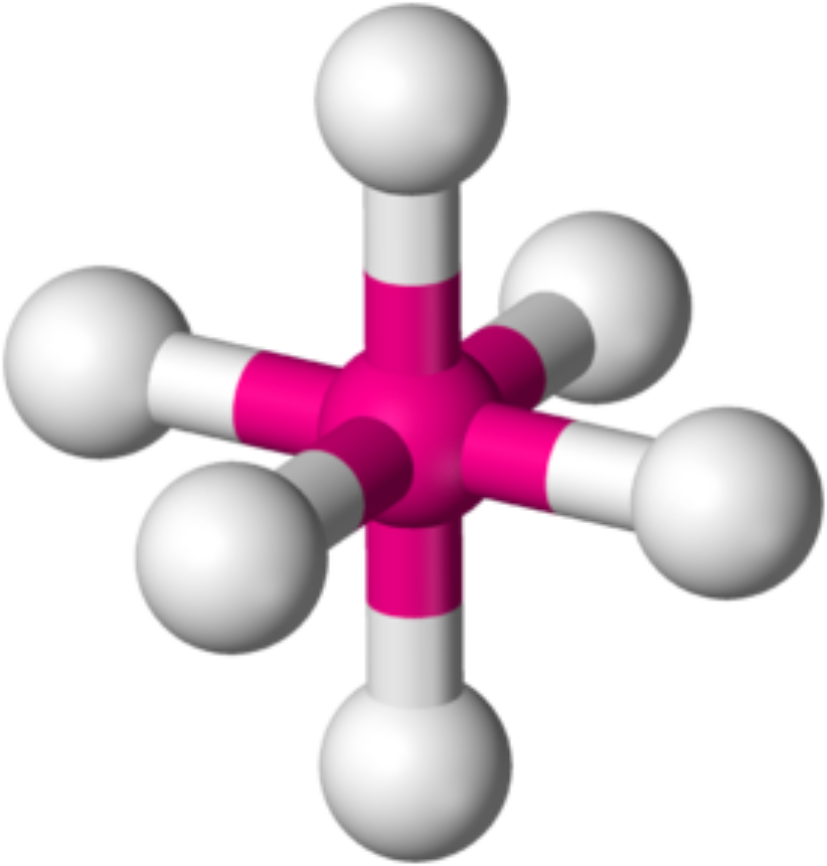
\includegraphics[scale=1]{AX6}}}$
		\hfill
		\cfig{
		S
		(<:[:20]H)
		(<[:-20]H)
		(-[2]H)
		(<:[:160]H)
		(<[:200]H)
		(-[6]H)
		}
		\hfill~
	\end{center}
\end{itemize}

\subsection{Polarité des liaisons et des molécules}
Les édifices moléculaires sont par essence des interactions entre particules
électriques. Il existe donc des champs électriques qui vont exercer des forces
de \textsc{Lorentz} et ils font donc partie intégrante des comportements entre
molécules.
\subsubsection{Électronégativité}
Le nombre d'électrons de valence ne permet pas de prédire toutes les évolutions
des propriétés chimiques que l'on constate expérimentalement. Dans les
molécules, les données expérimentales montrent que la distribution de charge
n'est pas symétrique. Certains atomes retiennent plus leurs électrons de valence
que d'autres.
\begin{tcb*}(defi){Électronégativité}
	\psw{
		Pour mesurer cette propriété, on définit l'électronégativité. Cette grandeur
		sans dimension, notée $\chi$, caractérise la \textbf{tendance d'un élément à
			attirer les électrons d'une liaison chimique}. Plus $\chi$ est grand, plus
		les électrons auront tendance à se rapprocher de l'élément.
	}
\end{tcb*}
On observe une certaine tendance dans les éléments chimiques en fonction de leur
position dans la classification~:
\begin{itemize}
	\bitem{Au sein d'une même période}~:
	\begin{itemize}
		\bitem{À gauche},
		\psw{
			les métaux alcalins et alcalino-terreux ont un électron de plus
			que le gaz rare qui les précède, et ils ont donc tendance à se
			\textbf{laisser prendre un électron} pour arriver à une
			configuration stable, ils sont \textbf{peu électronégatifs}.
		}
		\bitem{À droite},
		\psw{
			les halogènes vont chercher à
			\textbf{gagner un électron} pour avoir la configuration du gaz
			rare qui suit, et ils sont donc \textbf{très électronégatifs}.
		}
		\bitem{En général}, on garde cette tendance, et on
		pourra retenir~:
	\end{itemize}
\end{itemize}
\begin{tcb*}[cnt, bld](ror){Évolution de l'électronégativité dans une période}
	\psw{
		Au sein d'une période, l'électronégativité augmente de gauche à droite,
		avec le numéro atomique.
	}
\end{tcb*}
\begin{itemize}
	\bitem{Au sein d'une même famille}~:
	\begin{itemize}
		\bitem{En haut},
		\psw{
			les éléments ont de petits nuages
			électroniques, très reliés au noyau. Ils faut donc plus
			d'énergie pour leur arracher un électron, ou à l'inverse les
			électrons sont \textbf{très attirés} par les noyaux donc il y a
			une \textbf{grande électronégativité}~;
		}
		\bitem{En bas},
		\psw{
			les éléments ont des électrons de valence de
			plus en plus éloignés du noyau et donc de moins en moins
			reliés~: ces éléments \textbf{cèdent facilement} leurs
			électrons, et ils sont \textbf{peu électronégatifs}.
		}
		\bitem{En général}, on garde cette tendance, et on pourra retenir~:
	\end{itemize}
\end{itemize}
\begin{tcb*}[bld, cnt](ror){Évolution de l'électronégativité dans une famille}
	\psw{
		Au sein d'une famille, l'électronégativité augmente de bas en haut, vers
		les numéros atomiques décroissants
	}
\end{tcb*}
\begin{itemize}
	\bitem{Bilan qualitatif}~:
\end{itemize}
\begin{center}
	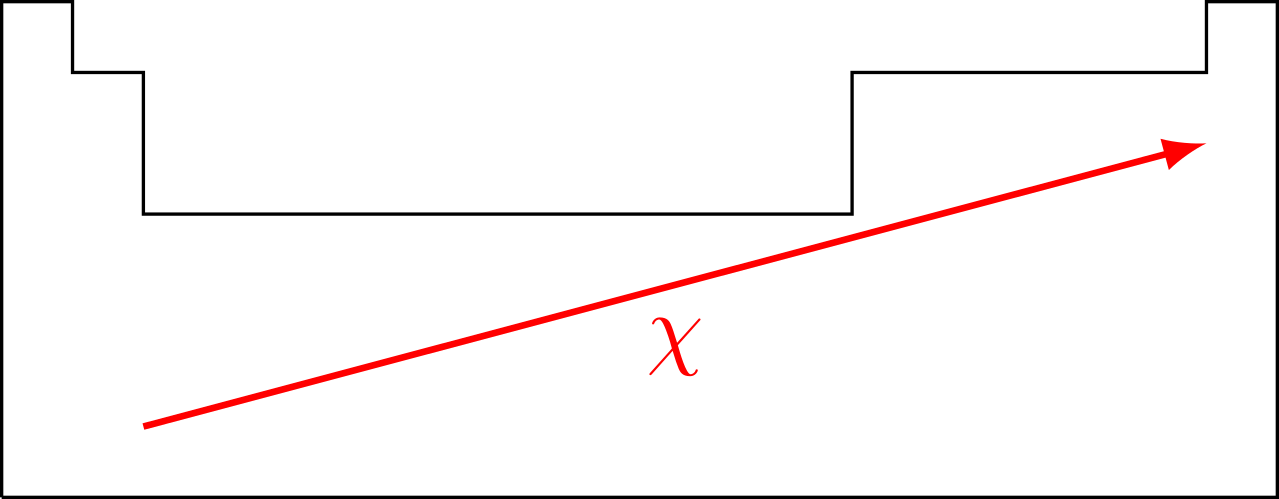
\includegraphics[scale=1]{elecnegtab}
\end{center}

\begin{tcb*}(rema)<lftt>'l'{Électrodéficience}
	\begin{itemize}
		\item Évidemment, des subtilités persistent.
		\item Il existe différentes échelles d'électronégativité, mais elle vaut
		      généralement entre 3 et 5 (pas d'unité).
		\item L'élément le plus électronégatif est le fluor ($\chi = \num{3.98}$
		      sur l'échelle de \textsc{Pauling}), le francium le moins
		      électronégatif ($\chi = \num{0.70}$).
	\end{itemize}
\end{tcb*}

\subsubsection{Moment dipolaire d'une liaison}

Le fait que certains atomes soient plus électronégatifs que d'autres implique
que les liaisons covalentes ne répartissent pas équitablement les électrons du
doublet liant~; en réalité, les atomes les \textbf{plus électronégatifs}
s'entourent un peu \textbf{plus d'électrons} que les autres.
\bigbreak
Ainsi, dans une molécule diatomique hétéronucléaire\ftn{Une molécule avec deux
	atomes A et B différents}, si $\chi_{\ce{A}} > \chi_{\ce{B}}$ alors A porte une
\textbf{charge partielle négative}, et B porte une \textbf{charge partielle
	positive} de même valeur absolue~:
\psw{
	\[
		\cfig{
			\charge{90=\|,180=\|,-90=\|,120:4pt=$-q$}{A}-
			\charge{60:4pt=$+q$}{B}
		}
	\]
}
En effet, \ce{A} attire davantage à lui les électrons de la liaison~: on dit que
la liaison est \textbf{polarisée}. Pour savoir à quel point les deux atomes sont
liés par liaison covalente, et non pas juste deux ions l'un à côté de l'autre,
on définit alors une grandeur~:

\begin{tcb*}[sidebyside](defi){Charge partielle et pourcentage d'ionicité}
	\psw{
		Des éléments \textbf{d'électronégativités différentes} attirent plus ou moins
		les électrons de la liaison, faisant apparaître des \textbf{charges
			partielles}, inférieures à la charge élémentaire.
		\bigbreak
		Les charges partielles sont
		d’autant plus grandes que les électronégativités sont différentes.
	}
	\tcblower
	Une charge partielle a pour valeur
	\psw{
		\[
			\boxed{q = \pm \delta e}
			\Lra
			\boxed{\de = \frac{\abs{q}}{e}}
		\]
	}
	avec $q$ la charge partielle, $e = \SI{1.602e-19}{C}$ la charge
	élémentaire, et $\delta$ le \textbf{pourcentage d'ionicité}, et se représente
	avec la notation
	\psw{
		\[
			\cfig{
				\charge{90=\|,180=\|,-90=\|,120:4pt=$\de-$}{A}-
				\charge{60:4pt=$\de+$}{B}
			}
		\]
	}
	\vspace{-15pt}
\end{tcb*}

Ainsi, l'atome le plus électronégatif porte la charge $-\de e$ et le plus
électronégatif la charge $+\de e$. Pour représenter géométriquement le champ
électrique créé par cette dissymétrie de charge, on introduit une grandeur
vectorielle~:

\begin{tcb*}[sidebyside, righthand ratio=.35](defi){Moment dipolaire}
	On appelle \textbf{moment dipolaire} $\muf$ (parfois $\pf$) d'une liaison le
	vecteur de caractéristiques suivantes~:
	\begin{itemize}
		\item \psw{
			      dirigé parallèlement à la liaison~;
		      }
		\item
		      \psw{
			      orienté de $-\de e$ à $+\de e$~;
		      }
		\item
		      \psw{
			      de norme $\ell\de e$ avec $\ell$ la longueur de la liaison
		      }
	\end{itemize}
	soit pour $\chi_{\ce{A}} > \chi_{\ce{B}}$~:
	\psw{
		\[
			\boxed{\muf_{\ce{A-B}} = q\ABf}
			\qquad \qquad
			\cfig{
				@{a}\charge{90=\|,180=\|,-90=\|,120:4pt=$\de-$}{A}-
				@{b}\charge{60:4pt=$\de+$}{B}
			}
			\chemmove[transform canvas={yshift=-10pt}]{
				\draw[-to]
				(a)--
				node[midway, below] {$\muf$}
				(b);
			}
		\]
	}
	\vspace{5pt}
	\tcblower
	\begin{center}
		\tcbsubtitle{\fatbox{Unité}}
	\end{center}
	Le moment dipolaire s'exprime en \textbf{\si{C.m}} en SI, ou usuellement en
	\textbf{Debye} D, tel que
	\[\SI{1}{D} = \frac{1}{3}\times\SI{e-29}{C.m}\]
\end{tcb*}

\begin{tcb*}(exem)<lftt>'l'{Moments dipolaires}
	\begin{itemize}
		\item Liaison \ce{O-H}~: $\norm{\muf} = \SI{1.51}{D}$
		\item Liaison \ce{C-H}~: $\norm{\muf} = \SI{0.4}{D}$. En effet,
		      $\chi_{\ce{C}} \approx \chi_{\ce{H}}$~: on pourra considérer
		      \ce{C-H} comme \textbf{apolaire} la plupart du temps.
	\end{itemize}
\end{tcb*}

\begin{tcb*}(appl)<lftt>'l'{Pourcentage d'ionicité}
	On donne la longueur de liaison et le moment dipolaire~: donner le
	pourcentage d'ionicité.
	\tcblower
	\begin{center}
		\centering
		\captionof{table}{Calcul de $\protect\de$ connaissant $\protect\ell$ et
			$\protect\norm{\protect\muf}$.}
		\label{tab:delpf}
		\begin{tabular}{cccc}
			\toprule
			Liaison   & Moment dipolaire (\si{D})   & Longueur de liaison (\si{pm})
			          & Pourcentage d'ionicité (\%)
			\\\midrule
			\ce{H-F}  & \num{1.82}                  & \num{92}                      & \psw{\num{41}} \\
			\ce{H-Cl} & \num{1.08}                  & \num{127}                     & \psw{\num{18}} \\
			\ce{H-Br} & \num{0.79}                  & \num{142}                     & \psw{\num{12}} \\
			\ce{H-I}  & \num{0.38}                  & \num{161}                     & \psw{\num{5}}  \\
			\bottomrule
		\end{tabular}
	\end{center}
\end{tcb*}

\subsubsection{Moment dipolaire d'une molécule}

\begin{tcb*}(defi){Moment dipolaire d'une molécule, polaire ou apolaire}
	Dans une molécule, le moment dipolaire total est la \textbf{somme
		vectorielle} des moments dipolaires des liaisons covalentes la constituant~:
	\psw{
		\[\boxed{\muf_{\rm tot} = \sum_i \muf_i}\]
	}
	Une molécule est donc dite \textbf{polaire} si son moment dipolaire total
	n'est pas nul, \textbf{apolaire} sinon.
\end{tcb*}

\begin{tcb*}(appl)<lftt>'l'{Moments dipolaires de molécules}
	\begin{itemize}
		\bitem{Le \ce{CO2}}~:
		\[
			\cfig{
				\charge{120=\|,-120=\|,-90:4pt=$\delta-$}{O}=
				\charge{-90:4pt=$2\delta +$}{C}=
				\charge{60=\|,-60=\|,-90:4pt=$\delta-$}{O}
			}
		\]
		\psw{
			Le moment dipolaire total est nul puisque les deux moments de
			\ce{C=O} se compensent.
		}
		\bitem{L'eau}~: à partir de $\mu_{\ce{O-H}} = \SI{1.51}{D}$ et connaissant
		l'angle $\widehat{(\rm HOH)} = \ang{104.45}$, calculer le moment
		dipolaire de l'eau
		\begin{center}
			\cfig{
				\lewis{13,O}
				(-[@{d}:-37.775]H)
				(-[@{g}:217.775]H)
			}
			\chemmove[to-to]{
				\draw
				(g) to[bend right]
				node [midway, below] {\ang{104.45}}
				(d)
				;}
		\end{center}
		\item[] \textbf{Méthode 1}~:
		      \psw{
			      on a
			      \[\muf = \muf_{\rm droite} + \muf_{\rm gauche}\]
			      avec
			      $\muf_{\rm droite} =
				      \mu_{\ce{OH}}\sin(\a/2)\ux +
				      \mu_{\ce{OH}}\cos(\a/2)\uy$, et
			      $\muf_{\rm gauche} =
				      -\mu_{\ce{OH}}\sin(\a/2)\ux +
				      \mu_{\ce{OH}}\cos(\a/2)\uy$~; ainsi
			      \begin{gather*}
				      \muf = 2\mu_{\ce{OH}}\cos(\a/2)\uy\\
				      \boxed{\mu_{\ce{H2O}} = 2\mu_{\ce{OH}}\cos(\a/2) = \SI{1.85}{D}}
			      \end{gather*}
		      }
		      \vspace{-15pt}
		\item[] \textbf{Méthode 2}~:
		      \psw{
			      on peut également raisonner dans le
			      triangle isocèle formé par les deux vecteurs issus de O~:
			      \begin{center}
				      \sswitch{
					      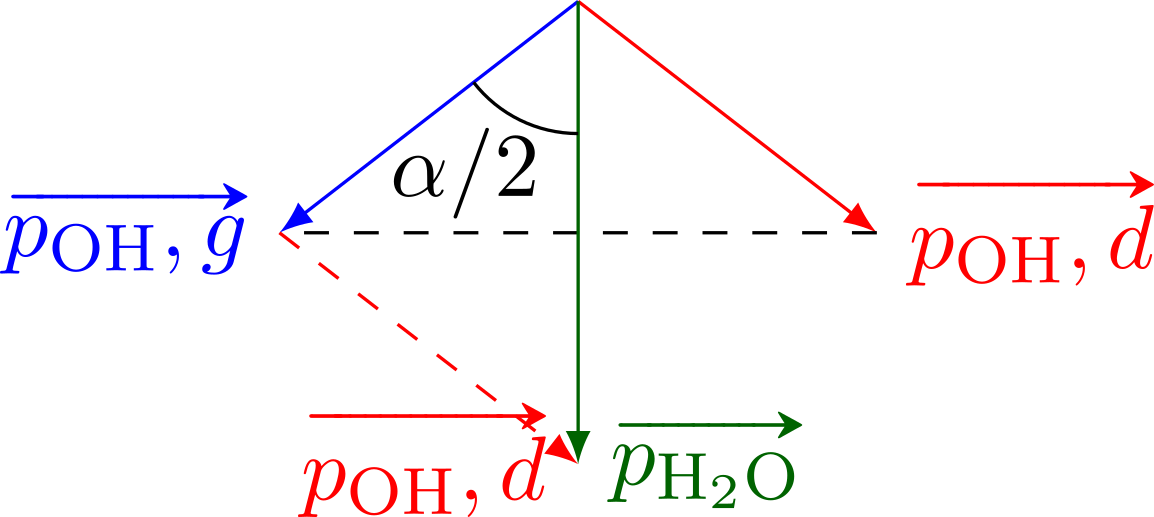
\includegraphics[scale=1, draft=true]{pH2O}
				      }{
					      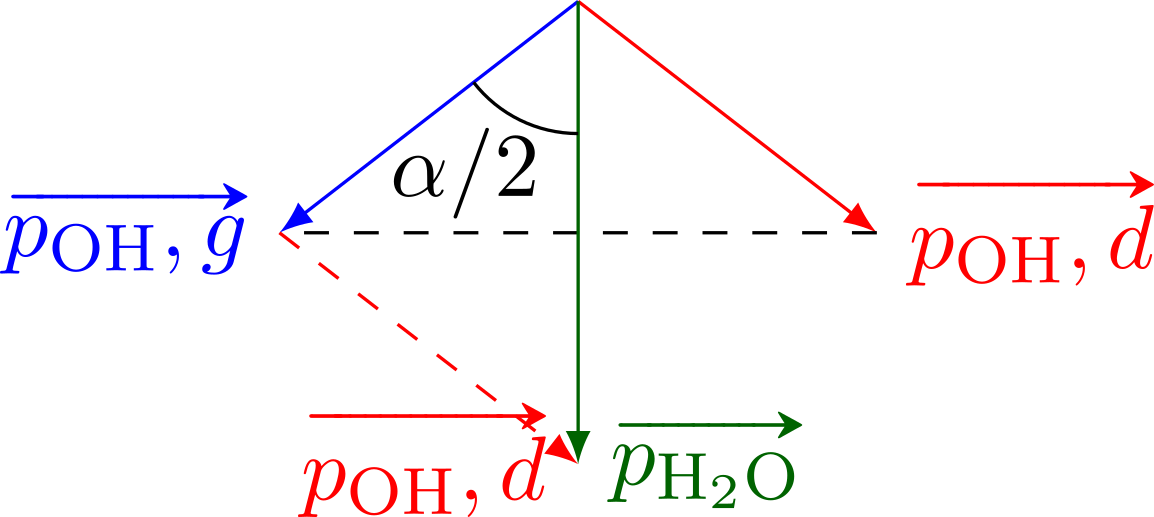
\includegraphics[scale=1]{pH2O}
				      }
			      \end{center}
			      \begin{gather*}
				      \beforetext{On a alors directement}
				      \cos(\frac{\a}{2}) = \frac{\mu_{\ce{H2O}}/2}{\mu_{\ce{OH}}}
			      \end{gather*}
		      }
	\end{itemize}
\end{tcb*}

\begin{tcb*}[cnt, bld](ror){Moment dipolaire d'une molécule symétrique}
	Par propriétés géométriques, une molécule à symétrie de rotation a un moment
	dipolaire nul.
\end{tcb*}

\subsubsection{Polarisabilité~: moment dipolaire induit}
En présence d'un champ électrique extérieur $\Ef_{\rm ext}$, une charge $q$
subit la force de \textsc{Lorentz} $\Ff_e = q\Ef_{\rm ext}$. La répartition des
charges d'un édifice électronique va donc changer~:
\begin{itemize}
	\item Les charges $+$ sont déplacées dans le sens de $\Ef_{\rm ext}$~;
	\item Les charges $-$ sont déplacées dans le sens opposé.
\end{itemize}
Ainsi, même en partant d'un édifice apolaire, l'action d'un champ extérieur
vient donner une dissymétrie aux charges.

\begin{tcb*}(defi){Moment dipolaire induit et polarisabilité}
	Sous l'action d'un champ $\Ef_{\rm ext}$, une liaison ou une molécule
	possède un \textbf{moment dipolaire induit} (par le champ), tel que
	\psw{
		\[\boxed{\muf = \a\Ef_{\rm ext}}\]
	}
	et on appelle $\a$ la \textbf{polarisabilité de la liaison}~: cette grandeur
	décrit la facilité d'un édifice à se déformer avec $\Ef$.
\end{tcb*}
\begin{tcb*}[cnt](ror){Polarisabilité}
	\psw{
		La polarisabilité d'une liaison augmente avec la «~taille~» des atomes
		liés et avec la multiplicité des liaisons~:
		\[
			\a_{\ce{C-C}} < \a_{\ce{C-F}} < \a_{\ce{C-Cl}}
			\qquad
			\a_{\ce{C-C}} < \a_{\ce{C=C}}
		\]
	}
	\vspace{-15pt}
\end{tcb*}
\begin{tcb*}(inte)<lftt>'l'{Polarisabilité}
	En effet, un noyau avec 2 électrons les attire chacun très fortement, et ils
	sont difficiles à déloger. À l'inverse, un noyau avec 82 électrons autour
	attire de moins en moins ceux qui sont le plus loin, non seulement par la
	distance mais aussi par effet d'écrantage des électrons situés sur les
	couches inférieures.
	\bigbreak
	De plus, même si les liaisons doubles sont plus courtes
	que les simples, elles sont plus facilement étirables puisqu'il y a plus
	d'électrons mis en jeu, donc une plus grande force \textsc{Lorentz} subie.
\end{tcb*}

% 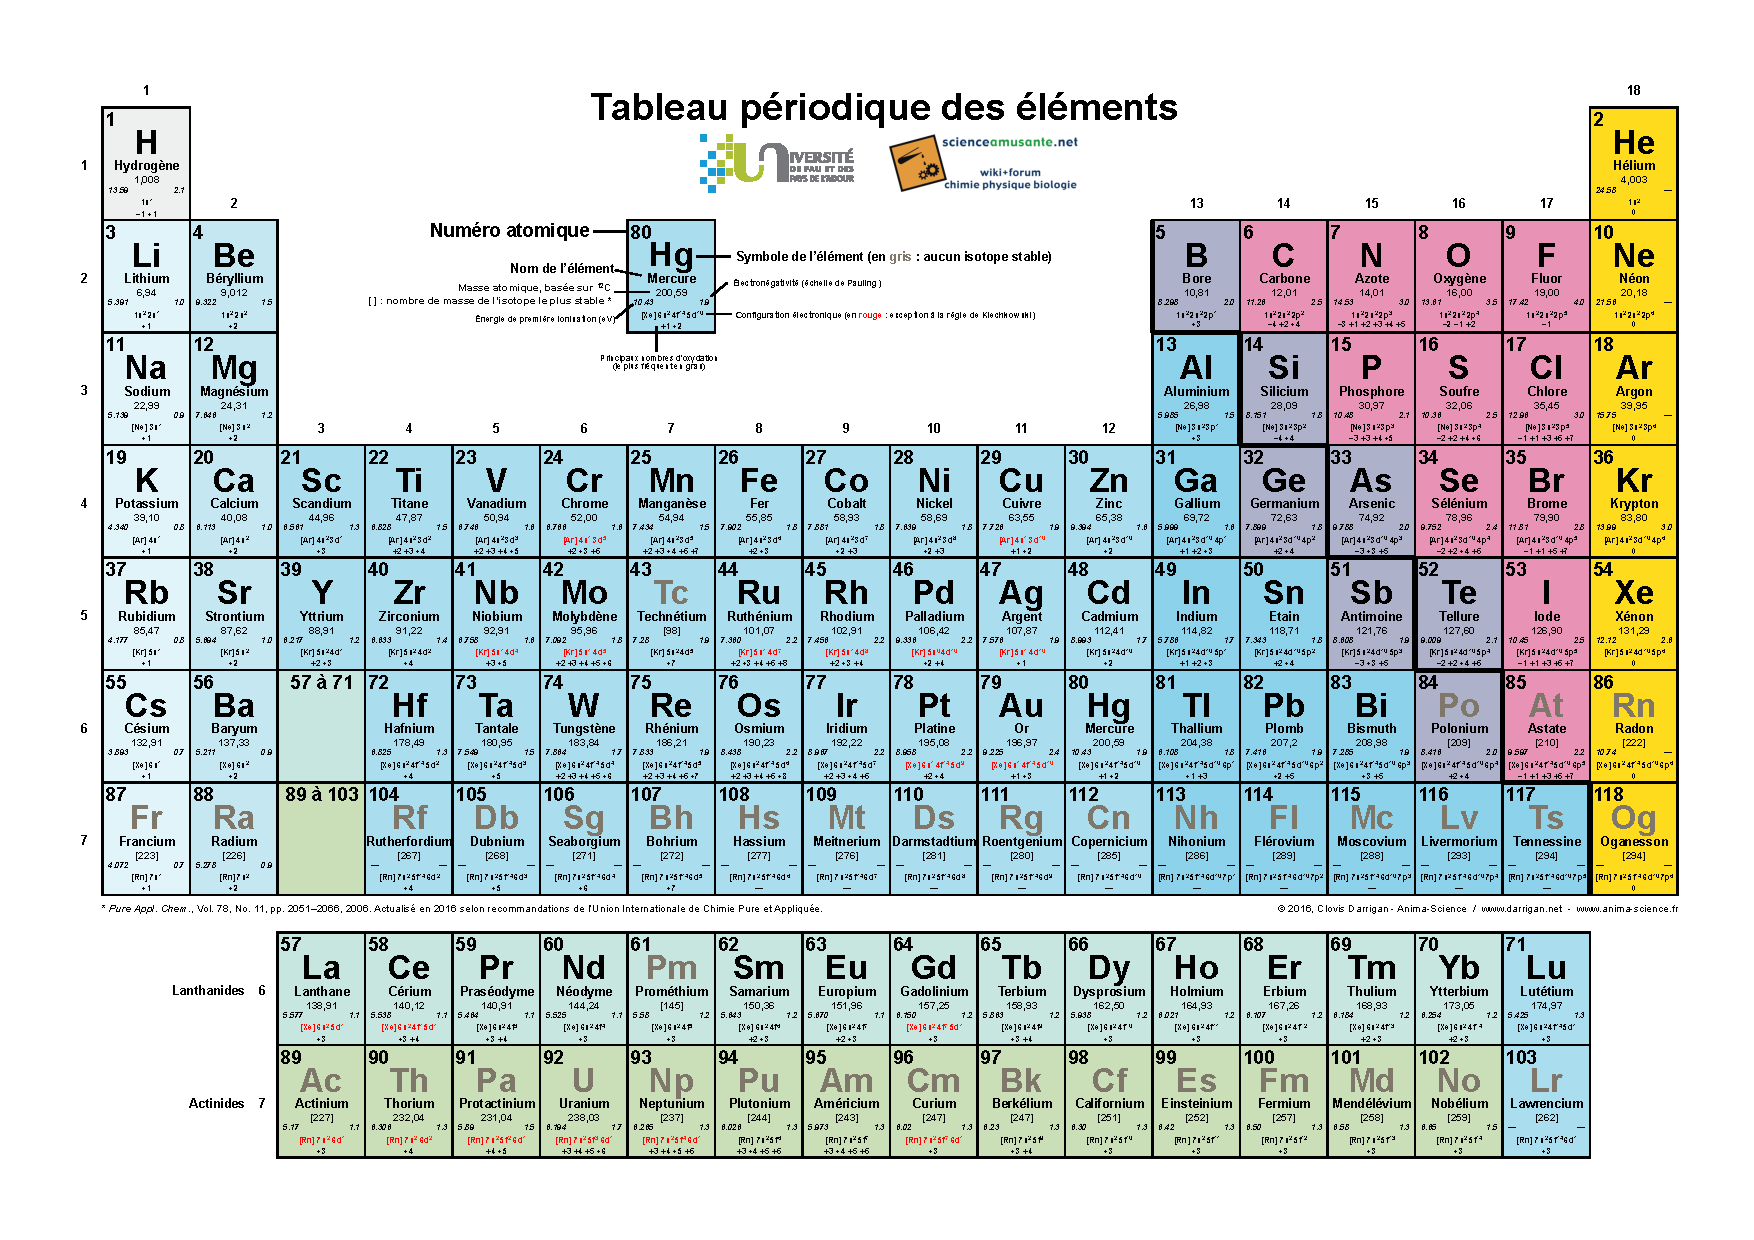
\includepdf[pages={-}, angle=90]{./figures/tab_peri_comp.pdf}

\end{document}
